% Options for packages loaded elsewhere
\PassOptionsToPackage{unicode}{hyperref}
\PassOptionsToPackage{hyphens}{url}
%
\documentclass[
]{article}
\usepackage{amsmath,amssymb}
\usepackage{iftex}
\ifPDFTeX
  \usepackage[T1]{fontenc}
  \usepackage[utf8]{inputenc}
  \usepackage{textcomp} % provide euro and other symbols
\else % if luatex or xetex
  \usepackage{unicode-math} % this also loads fontspec
  \defaultfontfeatures{Scale=MatchLowercase}
  \defaultfontfeatures[\rmfamily]{Ligatures=TeX,Scale=1}
\fi
\usepackage{lmodern}
\ifPDFTeX\else
  % xetex/luatex font selection
\fi
% Use upquote if available, for straight quotes in verbatim environments
\IfFileExists{upquote.sty}{\usepackage{upquote}}{}
\IfFileExists{microtype.sty}{% use microtype if available
  \usepackage[]{microtype}
  \UseMicrotypeSet[protrusion]{basicmath} % disable protrusion for tt fonts
}{}
\makeatletter
\@ifundefined{KOMAClassName}{% if non-KOMA class
  \IfFileExists{parskip.sty}{%
    \usepackage{parskip}
  }{% else
    \setlength{\parindent}{0pt}
    \setlength{\parskip}{6pt plus 2pt minus 1pt}}
}{% if KOMA class
  \KOMAoptions{parskip=half}}
\makeatother
\usepackage{xcolor}
\usepackage[margin=1in]{geometry}
\usepackage{color}
\usepackage{fancyvrb}
\newcommand{\VerbBar}{|}
\newcommand{\VERB}{\Verb[commandchars=\\\{\}]}
\DefineVerbatimEnvironment{Highlighting}{Verbatim}{commandchars=\\\{\}}
% Add ',fontsize=\small' for more characters per line
\usepackage{framed}
\definecolor{shadecolor}{RGB}{248,248,248}
\newenvironment{Shaded}{\begin{snugshade}}{\end{snugshade}}
\newcommand{\AlertTok}[1]{\textcolor[rgb]{0.94,0.16,0.16}{#1}}
\newcommand{\AnnotationTok}[1]{\textcolor[rgb]{0.56,0.35,0.01}{\textbf{\textit{#1}}}}
\newcommand{\AttributeTok}[1]{\textcolor[rgb]{0.13,0.29,0.53}{#1}}
\newcommand{\BaseNTok}[1]{\textcolor[rgb]{0.00,0.00,0.81}{#1}}
\newcommand{\BuiltInTok}[1]{#1}
\newcommand{\CharTok}[1]{\textcolor[rgb]{0.31,0.60,0.02}{#1}}
\newcommand{\CommentTok}[1]{\textcolor[rgb]{0.56,0.35,0.01}{\textit{#1}}}
\newcommand{\CommentVarTok}[1]{\textcolor[rgb]{0.56,0.35,0.01}{\textbf{\textit{#1}}}}
\newcommand{\ConstantTok}[1]{\textcolor[rgb]{0.56,0.35,0.01}{#1}}
\newcommand{\ControlFlowTok}[1]{\textcolor[rgb]{0.13,0.29,0.53}{\textbf{#1}}}
\newcommand{\DataTypeTok}[1]{\textcolor[rgb]{0.13,0.29,0.53}{#1}}
\newcommand{\DecValTok}[1]{\textcolor[rgb]{0.00,0.00,0.81}{#1}}
\newcommand{\DocumentationTok}[1]{\textcolor[rgb]{0.56,0.35,0.01}{\textbf{\textit{#1}}}}
\newcommand{\ErrorTok}[1]{\textcolor[rgb]{0.64,0.00,0.00}{\textbf{#1}}}
\newcommand{\ExtensionTok}[1]{#1}
\newcommand{\FloatTok}[1]{\textcolor[rgb]{0.00,0.00,0.81}{#1}}
\newcommand{\FunctionTok}[1]{\textcolor[rgb]{0.13,0.29,0.53}{\textbf{#1}}}
\newcommand{\ImportTok}[1]{#1}
\newcommand{\InformationTok}[1]{\textcolor[rgb]{0.56,0.35,0.01}{\textbf{\textit{#1}}}}
\newcommand{\KeywordTok}[1]{\textcolor[rgb]{0.13,0.29,0.53}{\textbf{#1}}}
\newcommand{\NormalTok}[1]{#1}
\newcommand{\OperatorTok}[1]{\textcolor[rgb]{0.81,0.36,0.00}{\textbf{#1}}}
\newcommand{\OtherTok}[1]{\textcolor[rgb]{0.56,0.35,0.01}{#1}}
\newcommand{\PreprocessorTok}[1]{\textcolor[rgb]{0.56,0.35,0.01}{\textit{#1}}}
\newcommand{\RegionMarkerTok}[1]{#1}
\newcommand{\SpecialCharTok}[1]{\textcolor[rgb]{0.81,0.36,0.00}{\textbf{#1}}}
\newcommand{\SpecialStringTok}[1]{\textcolor[rgb]{0.31,0.60,0.02}{#1}}
\newcommand{\StringTok}[1]{\textcolor[rgb]{0.31,0.60,0.02}{#1}}
\newcommand{\VariableTok}[1]{\textcolor[rgb]{0.00,0.00,0.00}{#1}}
\newcommand{\VerbatimStringTok}[1]{\textcolor[rgb]{0.31,0.60,0.02}{#1}}
\newcommand{\WarningTok}[1]{\textcolor[rgb]{0.56,0.35,0.01}{\textbf{\textit{#1}}}}
\usepackage{graphicx}
\makeatletter
\def\maxwidth{\ifdim\Gin@nat@width>\linewidth\linewidth\else\Gin@nat@width\fi}
\def\maxheight{\ifdim\Gin@nat@height>\textheight\textheight\else\Gin@nat@height\fi}
\makeatother
% Scale images if necessary, so that they will not overflow the page
% margins by default, and it is still possible to overwrite the defaults
% using explicit options in \includegraphics[width, height, ...]{}
\setkeys{Gin}{width=\maxwidth,height=\maxheight,keepaspectratio}
% Set default figure placement to htbp
\makeatletter
\def\fps@figure{htbp}
\makeatother
\setlength{\emergencystretch}{3em} % prevent overfull lines
\providecommand{\tightlist}{%
  \setlength{\itemsep}{0pt}\setlength{\parskip}{0pt}}
\setcounter{secnumdepth}{-\maxdimen} % remove section numbering
\ifLuaTeX
  \usepackage{selnolig}  % disable illegal ligatures
\fi
\IfFileExists{bookmark.sty}{\usepackage{bookmark}}{\usepackage{hyperref}}
\IfFileExists{xurl.sty}{\usepackage{xurl}}{} % add URL line breaks if available
\urlstyle{same}
\hypersetup{
  pdftitle={partition},
  hidelinks,
  pdfcreator={LaTeX via pandoc}}

\title{partition}
\author{}
\date{\vspace{-2.5em}2024-03-15}

\begin{document}
\maketitle

\hypertarget{partition-simple}{%
\section{Partition simple}\label{partition-simple}}

\begin{Shaded}
\begin{Highlighting}[]
\CommentTok{\#setwd("\textasciitilde{}/Repositories/cherry{-}stats/projets/LAL")}
\FunctionTok{load}\NormalTok{(}\StringTok{"qaly.RData"}\NormalTok{)}
\FunctionTok{library}\NormalTok{(dplyr)}
\end{Highlighting}
\end{Shaded}

\begin{verbatim}
## 
## Attachement du package : 'dplyr'
\end{verbatim}

\begin{verbatim}
## Les objets suivants sont masqués depuis 'package:stats':
## 
##     filter, lag
\end{verbatim}

\begin{verbatim}
## Les objets suivants sont masqués depuis 'package:base':
## 
##     intersect, setdiff, setequal, union
\end{verbatim}

\begin{Shaded}
\begin{Highlighting}[]
\FunctionTok{library}\NormalTok{(boot)}
\FunctionTok{library}\NormalTok{(survRM2)}
\end{Highlighting}
\end{Shaded}

\begin{verbatim}
## Le chargement a nécessité le package : survival
\end{verbatim}

\begin{verbatim}
## 
## Attachement du package : 'survival'
\end{verbatim}

\begin{verbatim}
## L'objet suivant est masqué depuis 'package:boot':
## 
##     aml
\end{verbatim}

\begin{Shaded}
\begin{Highlighting}[]
\NormalTok{qaly}\SpecialCharTok{$}\NormalTok{finctdt   }\OtherTok{\textless{}{-}} \FunctionTok{apply}\NormalTok{(qaly[,}\FunctionTok{c}\NormalTok{(}\StringTok{"C1dt"}\NormalTok{,}\StringTok{"C2dt"}\NormalTok{ , }\StringTok{"C3dt"}\NormalTok{ , }\StringTok{"C4dt"}\NormalTok{, }\StringTok{"Inter1dt"}\NormalTok{ )],}\DecValTok{1}\NormalTok{,max,}\AttributeTok{na.rm=}\NormalTok{T)}
\NormalTok{qaly}\SpecialCharTok{$}\NormalTok{finct.dt }\OtherTok{\textless{}{-}} \FunctionTok{as.Date}\NormalTok{(}\FunctionTok{as.character}\NormalTok{(qaly}\SpecialCharTok{$}\NormalTok{finctdt),}\AttributeTok{format=}\StringTok{"\%Y{-}\%m{-}\%d"}\NormalTok{)}
\end{Highlighting}
\end{Shaded}

\begin{Shaded}
\begin{Highlighting}[]
\NormalTok{qaly}\SpecialCharTok{$}\NormalTok{suivi  }\OtherTok{\textless{}{-}} \FunctionTok{as.numeric}\NormalTok{(qaly}\SpecialCharTok{$}\NormalTok{Datemax}\SpecialCharTok{{-}}\NormalTok{qaly}\SpecialCharTok{$}\NormalTok{randodt)}\SpecialCharTok{/}\NormalTok{(}\FloatTok{365.25}\SpecialCharTok{/}\DecValTok{12}\NormalTok{)}
\NormalTok{qaly}\SpecialCharTok{$}\NormalTok{survie }\OtherTok{\textless{}{-}} \FunctionTok{as.numeric}\NormalTok{(qaly}\SpecialCharTok{$}\NormalTok{deathdt}\SpecialCharTok{{-}}\NormalTok{qaly}\SpecialCharTok{$}\NormalTok{randodt)}\SpecialCharTok{/}\NormalTok{(}\FloatTok{365.25}\SpecialCharTok{/}\DecValTok{12}\NormalTok{)}
\NormalTok{qaly}\SpecialCharTok{$}\NormalTok{delfinct }\OtherTok{\textless{}{-}} \FunctionTok{as.numeric}\NormalTok{(qaly}\SpecialCharTok{$}\NormalTok{finct.dt}\SpecialCharTok{{-}}\NormalTok{qaly}\SpecialCharTok{$}\NormalTok{randodt)}\SpecialCharTok{/}\NormalTok{(}\FloatTok{365.25}\SpecialCharTok{/}\DecValTok{12}\NormalTok{)}
\NormalTok{qaly}\SpecialCharTok{$}\NormalTok{delarr }\OtherTok{\textless{}{-}} \FunctionTok{as.numeric}\NormalTok{(qaly}\SpecialCharTok{$}\NormalTok{arrpremadt}\SpecialCharTok{{-}}\NormalTok{qaly}\SpecialCharTok{$}\NormalTok{randodt)}\SpecialCharTok{/}\NormalTok{(}\FloatTok{365.25}\SpecialCharTok{/}\DecValTok{12}\NormalTok{)}
\NormalTok{qaly}\SpecialCharTok{$}\NormalTok{delfinct[}\FunctionTok{which}\NormalTok{(qaly}\SpecialCharTok{$}\NormalTok{delfinct}\SpecialCharTok{==}\DecValTok{0}\NormalTok{)]}\OtherTok{\textless{}{-}}\NormalTok{ qaly}\SpecialCharTok{$}\NormalTok{delarr[}\FunctionTok{which}\NormalTok{(qaly}\SpecialCharTok{$}\NormalTok{delfinct}\SpecialCharTok{==}\DecValTok{0}\NormalTok{)]}
\NormalTok{qaly}\SpecialCharTok{$}\NormalTok{finct}\OtherTok{\textless{}{-}} \FunctionTok{rep}\NormalTok{(}\DecValTok{1}\NormalTok{,}\FunctionTok{length}\NormalTok{(qaly}\SpecialCharTok{$}\NormalTok{delfinct))}
\NormalTok{qaly}\SpecialCharTok{$}\NormalTok{delrec}\OtherTok{\textless{}{-}} \FunctionTok{as.numeric}\NormalTok{(qaly}\SpecialCharTok{$}\NormalTok{relapsdt}\SpecialCharTok{{-}}\NormalTok{qaly}\SpecialCharTok{$}\NormalTok{randodt)}\SpecialCharTok{/}\NormalTok{(}\FloatTok{365.25}\SpecialCharTok{/}\DecValTok{12}\NormalTok{)}
\NormalTok{qaly}\SpecialCharTok{$}\NormalTok{delpfs}\OtherTok{\textless{}{-}}\NormalTok{ qaly}\SpecialCharTok{$}\NormalTok{suivi}
\NormalTok{qaly}\SpecialCharTok{$}\NormalTok{delpfs[}\SpecialCharTok{!}\FunctionTok{is.na}\NormalTok{(qaly}\SpecialCharTok{$}\NormalTok{delrec)]}\OtherTok{\textless{}{-}}\NormalTok{qaly}\SpecialCharTok{$}\NormalTok{delrec[}\SpecialCharTok{!}\FunctionTok{is.na}\NormalTok{(qaly}\SpecialCharTok{$}\NormalTok{delrec)]}
\NormalTok{qaly}\SpecialCharTok{$}\NormalTok{delbmt }\OtherTok{\textless{}{-}} \FunctionTok{as.numeric}\NormalTok{(qaly}\SpecialCharTok{$}\NormalTok{bmtdt}\SpecialCharTok{{-}}\NormalTok{qaly}\SpecialCharTok{$}\NormalTok{randodt)}\SpecialCharTok{/}\NormalTok{(}\FloatTok{365.25}\SpecialCharTok{/}\DecValTok{12}\NormalTok{)}
\NormalTok{qaly}\SpecialCharTok{$}\NormalTok{delbmt1 }\OtherTok{\textless{}{-}} \FunctionTok{as.numeric}\NormalTok{(qaly}\SpecialCharTok{$}\NormalTok{cgvhdt}\SpecialCharTok{{-}}\NormalTok{qaly}\SpecialCharTok{$}\NormalTok{randodt)}\SpecialCharTok{/}\NormalTok{(}\FloatTok{365.25}\SpecialCharTok{/}\DecValTok{12}\NormalTok{)}
\NormalTok{qaly}\SpecialCharTok{$}\NormalTok{delbmt2 }\OtherTok{\textless{}{-}} \FunctionTok{as.numeric}\NormalTok{(qaly}\SpecialCharTok{$}\NormalTok{agvhdt}\SpecialCharTok{{-}}\NormalTok{qaly}\SpecialCharTok{$}\NormalTok{randodt)}\SpecialCharTok{/}\NormalTok{(}\FloatTok{365.25}\SpecialCharTok{/}\DecValTok{12}\NormalTok{)}

\NormalTok{qaly}\SpecialCharTok{$}\NormalTok{delfinct2 }\OtherTok{\textless{}{-}}\NormalTok{ qaly}\SpecialCharTok{$}\NormalTok{delfinct}
\NormalTok{qaly}\SpecialCharTok{$}\NormalTok{delfinct2[}\SpecialCharTok{!}\FunctionTok{is.na}\NormalTok{(qaly}\SpecialCharTok{$}\NormalTok{delbmt)]}\OtherTok{\textless{}{-}}\FunctionTok{pmax}\NormalTok{(qaly}\SpecialCharTok{$}\NormalTok{delfinct[}\SpecialCharTok{!}\FunctionTok{is.na}\NormalTok{(qaly}\SpecialCharTok{$}\NormalTok{delbmt)],qaly}\SpecialCharTok{$}\NormalTok{delbmt[}\SpecialCharTok{!}\FunctionTok{is.na}\NormalTok{(qaly}\SpecialCharTok{$}\NormalTok{delbmt)]) }\CommentTok{\#add ,qaly$delbmt1[!is.na(qaly$delbmt1)],qaly$delbmt2[!is.na(qaly$delbmt2)]}
\CommentTok{\#It takes in account the complication ecountered after the transplant}
\CommentTok{\#finct}
\NormalTok{qaly}\SpecialCharTok{$}\NormalTok{finct2 }\OtherTok{\textless{}{-}}\NormalTok{ qaly}\SpecialCharTok{$}\NormalTok{finct}
\NormalTok{qaly}\SpecialCharTok{$}\NormalTok{finct2[}\SpecialCharTok{!}\FunctionTok{is.na}\NormalTok{(qaly}\SpecialCharTok{$}\NormalTok{delbmt)]}\OtherTok{\textless{}{-}}\DecValTok{1}
\end{Highlighting}
\end{Shaded}

\hypertarget{compute-the-survival-curves-for-each-arm}{%
\subsubsection{Compute the survival curves for each
arm}\label{compute-the-survival-curves-for-each-arm}}

\begin{Shaded}
\begin{Highlighting}[]
\FunctionTok{library}\NormalTok{(survival)}

\CommentTok{\# Arm A}
\NormalTok{ct\_A  }\OtherTok{\textless{}{-}} \FunctionTok{survfit}\NormalTok{(}\FunctionTok{Surv}\NormalTok{(delfinct,finct)}\SpecialCharTok{\textasciitilde{}}\DecValTok{1}\NormalTok{,}\AttributeTok{data=}\NormalTok{qaly,}\AttributeTok{subset =}\NormalTok{ (R1 }\SpecialCharTok{==} \StringTok{"Intensive arm (A)"}\NormalTok{)) }\CommentTok{\# ct : Durée du traitement}
\NormalTok{ct2\_A  }\OtherTok{\textless{}{-}} \FunctionTok{survfit}\NormalTok{(}\FunctionTok{Surv}\NormalTok{(delfinct2,finct2)}\SpecialCharTok{\textasciitilde{}}\DecValTok{1}\NormalTok{,}\AttributeTok{data=}\NormalTok{qaly,}\AttributeTok{subset =}\NormalTok{ (R1 }\SpecialCharTok{==} \StringTok{"Intensive arm (A)"}\NormalTok{)) }\CommentTok{\#Durée du traitement avec complications}
\NormalTok{sv\_A  }\OtherTok{\textless{}{-}} \FunctionTok{survfit}\NormalTok{(}\FunctionTok{Surv}\NormalTok{(suivi,}\FunctionTok{as.numeric}\NormalTok{(}\FunctionTok{as.character}\NormalTok{(dc)))}\SpecialCharTok{\textasciitilde{}}\DecValTok{1}\NormalTok{,}\AttributeTok{data=}\NormalTok{qaly,}\AttributeTok{subset =}\NormalTok{ (R1 }\SpecialCharTok{==} \StringTok{"Intensive arm (A)"}\NormalTok{)) }\CommentTok{\# Durée de survie : Temps avant décès}
\NormalTok{efs\_A }\OtherTok{\textless{}{-}} \FunctionTok{survfit}\NormalTok{(}\FunctionTok{Surv}\NormalTok{(delpfs,}\FunctionTok{as.numeric}\NormalTok{(}\FunctionTok{as.character}\NormalTok{(pfs)))}\SpecialCharTok{\textasciitilde{}}\DecValTok{1}\NormalTok{, }\AttributeTok{data=}\NormalTok{qaly,}\AttributeTok{subset =}\NormalTok{ (R1 }\SpecialCharTok{==} \StringTok{"Intensive arm (A)"}\NormalTok{)) }\CommentTok{\# Durée de survie sans progression : Temps avant rechute }

\CommentTok{\# Arm B}
\NormalTok{ct\_B  }\OtherTok{\textless{}{-}} \FunctionTok{survfit}\NormalTok{(}\FunctionTok{Surv}\NormalTok{(delfinct,finct)}\SpecialCharTok{\textasciitilde{}}\DecValTok{1}\NormalTok{,}\AttributeTok{data=}\NormalTok{qaly,}\AttributeTok{subset =}\NormalTok{ (R1 }\SpecialCharTok{==} \StringTok{"Light arm (B)"}\NormalTok{))}
\NormalTok{ct2\_B  }\OtherTok{\textless{}{-}} \FunctionTok{survfit}\NormalTok{(}\FunctionTok{Surv}\NormalTok{(delfinct2,finct2)}\SpecialCharTok{\textasciitilde{}}\DecValTok{1}\NormalTok{,}\AttributeTok{data=}\NormalTok{qaly,}\AttributeTok{subset =}\NormalTok{ (R1 }\SpecialCharTok{==} \StringTok{"Light arm (B)"}\NormalTok{))}
\NormalTok{sv\_B  }\OtherTok{\textless{}{-}} \FunctionTok{survfit}\NormalTok{(}\FunctionTok{Surv}\NormalTok{(suivi,}\FunctionTok{as.numeric}\NormalTok{(}\FunctionTok{as.character}\NormalTok{(dc)))}\SpecialCharTok{\textasciitilde{}}\DecValTok{1}\NormalTok{,}\AttributeTok{data=}\NormalTok{qaly,}\AttributeTok{subset =}\NormalTok{ (R1 }\SpecialCharTok{==} \StringTok{"Light arm (B)"}\NormalTok{))}
\NormalTok{efs\_B }\OtherTok{\textless{}{-}} \FunctionTok{survfit}\NormalTok{(}\FunctionTok{Surv}\NormalTok{(delpfs,}\FunctionTok{as.numeric}\NormalTok{(}\FunctionTok{as.character}\NormalTok{(pfs)))}\SpecialCharTok{\textasciitilde{}}\DecValTok{1}\NormalTok{, }\AttributeTok{data=}\NormalTok{qaly,}\AttributeTok{subset =}\NormalTok{ (R1 }\SpecialCharTok{==} \StringTok{"Light arm (B)"}\NormalTok{))}
\end{Highlighting}
\end{Shaded}

\hypertarget{plot-the-survival-curves-for-each-arm}{%
\subsection{Plot the survival curves for each
arm}\label{plot-the-survival-curves-for-each-arm}}

\hypertarget{bras-a}{%
\subsubsection{Bras A}\label{bras-a}}

\begin{Shaded}
\begin{Highlighting}[]
\CommentTok{\#fig.width=6, fig.height=5.5 =\textgreater{} use later for website}

\NormalTok{fit1}\OtherTok{\textless{}{-}}\FunctionTok{list}\NormalTok{(}\AttributeTok{CT =}\NormalTok{ ct\_A, }\AttributeTok{CT2=}\NormalTok{ct2\_A,}\AttributeTok{SV=}\NormalTok{sv\_A, }\AttributeTok{EFS=}\NormalTok{efs\_A)}
\FunctionTok{library}\NormalTok{(survminer)}
\end{Highlighting}
\end{Shaded}

\begin{verbatim}
## Le chargement a nécessité le package : ggplot2
\end{verbatim}

\begin{verbatim}
## Le chargement a nécessité le package : ggpubr
\end{verbatim}

\begin{verbatim}
## 
## Attachement du package : 'survminer'
\end{verbatim}

\begin{verbatim}
## L'objet suivant est masqué depuis 'package:survival':
## 
##     myeloma
\end{verbatim}

\begin{Shaded}
\begin{Highlighting}[]
\FunctionTok{library}\NormalTok{(gridExtra)}
\end{Highlighting}
\end{Shaded}

\begin{verbatim}
## 
## Attachement du package : 'gridExtra'
\end{verbatim}

\begin{verbatim}
## L'objet suivant est masqué depuis 'package:dplyr':
## 
##     combine
\end{verbatim}

\begin{Shaded}
\begin{Highlighting}[]
\NormalTok{colors }\OtherTok{\textless{}{-}} \FunctionTok{c}\NormalTok{(}\StringTok{"\#A31621"}\NormalTok{, }\StringTok{"\#053C5E"}\NormalTok{, }\StringTok{"\#F3A712"}\NormalTok{, }\StringTok{"\#1F7A8C"}\NormalTok{, }\StringTok{"\#AFB3F7"}\NormalTok{)}

\NormalTok{t}\OtherTok{\textless{}{-}}\FunctionTok{ggsurvplot\_combine}\NormalTok{(fit1,}
          \AttributeTok{risk.table =} \ConstantTok{TRUE}\NormalTok{,                  }\CommentTok{\# Add risk table}
   \AttributeTok{xlab =} \StringTok{"Time in days"}\NormalTok{,   }\CommentTok{\# customize X axis label.}
   \AttributeTok{ggtheme =} \FunctionTok{theme\_light}\NormalTok{(), }\CommentTok{\# customize plot and risk table with a therme.}
 \AttributeTok{risk.table.y.text.col =}\NormalTok{ T, }\CommentTok{\# colour risk table text annotations.}
  \AttributeTok{risk.table.y.text =} \ConstantTok{FALSE}\NormalTok{,}
  \AttributeTok{legend.labs =} \FunctionTok{c}\NormalTok{(}\StringTok{"CT"}\NormalTok{,}\StringTok{"CT2"}\NormalTok{,}\StringTok{"SV"}\NormalTok{,}\StringTok{"EFS"}\NormalTok{))}
\end{Highlighting}
\end{Shaded}

\begin{verbatim}
## Warning: There was 1 warning in `mutate()`.
## i In argument: `survtable = purrr::map2(...)`.
## Caused by warning:
## ! `select_()` was deprecated in dplyr 0.7.0.
## i Please use `select()` instead.
## i The deprecated feature was likely used in the survminer package.
##   Please report the issue at <https://github.com/kassambara/survminer/issues>.
\end{verbatim}

\begin{Shaded}
\begin{Highlighting}[]
\NormalTok{sv\_plot\_A }\OtherTok{\textless{}{-}} \FunctionTok{ggsurvplot}\NormalTok{(sv\_A, }\AttributeTok{risk.table =} \ConstantTok{TRUE}\NormalTok{,}
                      \AttributeTok{ggtheme =} \FunctionTok{theme\_light}\NormalTok{(),}
                      \CommentTok{\# tables.theme = theme(}
                      \CommentTok{\#   axis.text.x = element\_blank(),  \# Hide x{-}axis text}
                      \CommentTok{\#   axis.ticks.x = element\_blank(), \# Hide x{-}axis ticks}
                      \CommentTok{\#   axis.title.x = element\_blank()  \# Optionally, hide the x{-}axis title as well}
                      \CommentTok{\# ),}
                      \AttributeTok{risk.table.y.text.col =} \ConstantTok{TRUE}\NormalTok{,}
                      \AttributeTok{risk.table.y.text =} \ConstantTok{FALSE}\NormalTok{,}
                      \AttributeTok{palette =}\NormalTok{ colors[}\DecValTok{2}\NormalTok{])  }

\FunctionTok{library}\NormalTok{(dplyr)}
\FunctionTok{library}\NormalTok{(gt)}
\FunctionTok{library}\NormalTok{(gtsummary)}
\FunctionTok{library}\NormalTok{(ks)}
\FunctionTok{library}\NormalTok{(tidyr)}
\FunctionTok{library}\NormalTok{(survival)}
\FunctionTok{library}\NormalTok{(ggplot2)}
\FunctionTok{library}\NormalTok{(ggsurvfit)}


\NormalTok{df}\OtherTok{\textless{}{-}}\NormalTok{t}\SpecialCharTok{$}\NormalTok{plot}\SpecialCharTok{$}\NormalTok{data}
\NormalTok{surv\_A}\OtherTok{\textless{}{-}}\NormalTok{df }\SpecialCharTok{\%\textgreater{}\%} \FunctionTok{mutate}\NormalTok{(}\AttributeTok{strata =} \FunctionTok{sub}\NormalTok{(}\StringTok{"x="}\NormalTok{, }\StringTok{""}\NormalTok{, strata)) }\SpecialCharTok{\%\textgreater{}\%}
  \FunctionTok{group\_by}\NormalTok{(strata) }\SpecialCharTok{\%\textgreater{}\%}
  \FunctionTok{summarise}\NormalTok{(}\AttributeTok{time =} \FunctionTok{c}\NormalTok{(time }\SpecialCharTok{{-}} \FloatTok{0.001}\NormalTok{, time),}
            \AttributeTok{surv =} \FunctionTok{c}\NormalTok{(}\DecValTok{1}\NormalTok{, }\FunctionTok{head}\NormalTok{(surv, }\SpecialCharTok{{-}}\DecValTok{1}\NormalTok{), surv),}
            \AttributeTok{.groups =} \StringTok{"drop"}\NormalTok{) }\SpecialCharTok{\%\textgreater{}\%}
  \FunctionTok{arrange}\NormalTok{(time) }\SpecialCharTok{\%\textgreater{}\%}
  \FunctionTok{pivot\_wider}\NormalTok{(}\AttributeTok{names\_from =} \StringTok{"strata"}\NormalTok{, }\AttributeTok{values\_from =} \StringTok{"surv"}\NormalTok{) }\SpecialCharTok{\%\textgreater{}\%}
  \FunctionTok{fill}\NormalTok{(}\DecValTok{1}\SpecialCharTok{:}\DecValTok{5}\NormalTok{, }\AttributeTok{.direction =} \StringTok{"downup"}\NormalTok{) }\SpecialCharTok{\%\textgreater{}\%}
  \FunctionTok{ggplot}\NormalTok{(}\FunctionTok{aes}\NormalTok{(time, CT)) }\SpecialCharTok{+}
  \FunctionTok{geom\_step}\NormalTok{(}\FunctionTok{aes}\NormalTok{(}\AttributeTok{linetype =} \StringTok{"CT"}\NormalTok{)) }\SpecialCharTok{+}
  \FunctionTok{geom\_ribbon}\NormalTok{(}\FunctionTok{aes}\NormalTok{(}\AttributeTok{ymin =} \DecValTok{0}\NormalTok{, }\AttributeTok{ymax =}\NormalTok{ CT, }\AttributeTok{fill =} \StringTok{"TOX1"}\NormalTok{),}\AttributeTok{alpha=}\FloatTok{0.5}\NormalTok{)}\SpecialCharTok{+}
  \FunctionTok{geom\_step}\NormalTok{(}\FunctionTok{aes}\NormalTok{(}\AttributeTok{y =}\NormalTok{ CT2, }\AttributeTok{linetype =} \StringTok{"CT2"}\NormalTok{),}\AttributeTok{linewidth=}\FloatTok{0.9}\NormalTok{, }\AttributeTok{colour=}\StringTok{"\#0077b6"}\NormalTok{) }\SpecialCharTok{+}
  \FunctionTok{geom\_ribbon}\NormalTok{(}\FunctionTok{aes}\NormalTok{(}\AttributeTok{ymin =}\NormalTok{ CT, }\AttributeTok{ymax =}\NormalTok{ CT2, }\AttributeTok{fill =} \StringTok{"TOX2"}\NormalTok{),}\AttributeTok{alpha=}\FloatTok{0.5}\NormalTok{) }\SpecialCharTok{+}
  \FunctionTok{geom\_step}\NormalTok{(}\FunctionTok{aes}\NormalTok{(}\AttributeTok{y =}\NormalTok{ EFS,}\AttributeTok{linetype =} \StringTok{"EFS"}\NormalTok{),}\AttributeTok{linewidth=}\FloatTok{0.9}\NormalTok{, }\AttributeTok{colour=}\StringTok{"\#48cae4"}\NormalTok{) }\SpecialCharTok{+}
  \FunctionTok{geom\_ribbon}\NormalTok{(}\FunctionTok{aes}\NormalTok{(}\AttributeTok{ymin =}\NormalTok{ CT2, }\AttributeTok{ymax =}\NormalTok{ EFS, }\AttributeTok{fill =} \StringTok{"TWiST"}\NormalTok{),}\AttributeTok{alpha=}\FloatTok{0.5}\NormalTok{)}\SpecialCharTok{+}
  \FunctionTok{geom\_step}\NormalTok{(}\FunctionTok{aes}\NormalTok{(}\AttributeTok{y =}\NormalTok{ SV,}\AttributeTok{linetype =} \StringTok{"SV"}\NormalTok{),}\AttributeTok{linewidth=}\FloatTok{0.9}\NormalTok{, }\AttributeTok{colour=}\StringTok{"\#caf0f8"}\NormalTok{)}\SpecialCharTok{+}
  \FunctionTok{geom\_ribbon}\NormalTok{(}\FunctionTok{aes}\NormalTok{(}\AttributeTok{ymin =}\NormalTok{ EFS, }\AttributeTok{ymax =}\NormalTok{ SV, }\AttributeTok{fill =} \StringTok{"REL"}\NormalTok{),}\AttributeTok{alpha=}\FloatTok{0.5}\NormalTok{)}\SpecialCharTok{+}
  \FunctionTok{scale\_fill\_manual}\NormalTok{(}\AttributeTok{values =} \FunctionTok{c}\NormalTok{(}\StringTok{"TOX1"} \OtherTok{=} \StringTok{"\#03045e"}\NormalTok{, }\StringTok{"TOX2"} \OtherTok{=} \StringTok{"\#0077b6"}\NormalTok{, }\StringTok{"TWiST"} \OtherTok{=} \StringTok{"\#48cae4"}\NormalTok{, }\StringTok{"REL"} \OtherTok{=} \StringTok{"\#caf0f8"}\NormalTok{)) }\SpecialCharTok{+}
  \FunctionTok{labs}\NormalTok{(}\AttributeTok{x =} \StringTok{"Time"}\NormalTok{, }\AttributeTok{y =} \StringTok{"Survival Probability"}\NormalTok{, }\AttributeTok{linetype =} \StringTok{"Duration"}\NormalTok{, }\AttributeTok{fill =} \StringTok{"Events"}\NormalTok{) }\SpecialCharTok{+}
  \FunctionTok{theme\_minimal}\NormalTok{() }\SpecialCharTok{+}
  \FunctionTok{theme}\NormalTok{(}\AttributeTok{legend.position =} \StringTok{"right"}\NormalTok{)}
\end{Highlighting}
\end{Shaded}

\begin{verbatim}
## Warning: Returning more (or less) than 1 row per `summarise()` group was deprecated in
## dplyr 1.1.0.
## i Please use `reframe()` instead.
## i When switching from `summarise()` to `reframe()`, remember that `reframe()`
##   always returns an ungrouped data frame and adjust accordingly.
## Call `lifecycle::last_lifecycle_warnings()` to see where this warning was
## generated.
\end{verbatim}

\begin{Shaded}
\begin{Highlighting}[]
\NormalTok{combined\_plot }\OtherTok{\textless{}{-}} \FunctionTok{grid.arrange}\NormalTok{(surv\_A, sv\_plot\_A}\SpecialCharTok{$}\NormalTok{table, }\AttributeTok{ncol =} \DecValTok{1}\NormalTok{,}\AttributeTok{heights =} \FunctionTok{c}\NormalTok{(}\DecValTok{6}\NormalTok{, }\DecValTok{2}\NormalTok{))}
\end{Highlighting}
\end{Shaded}

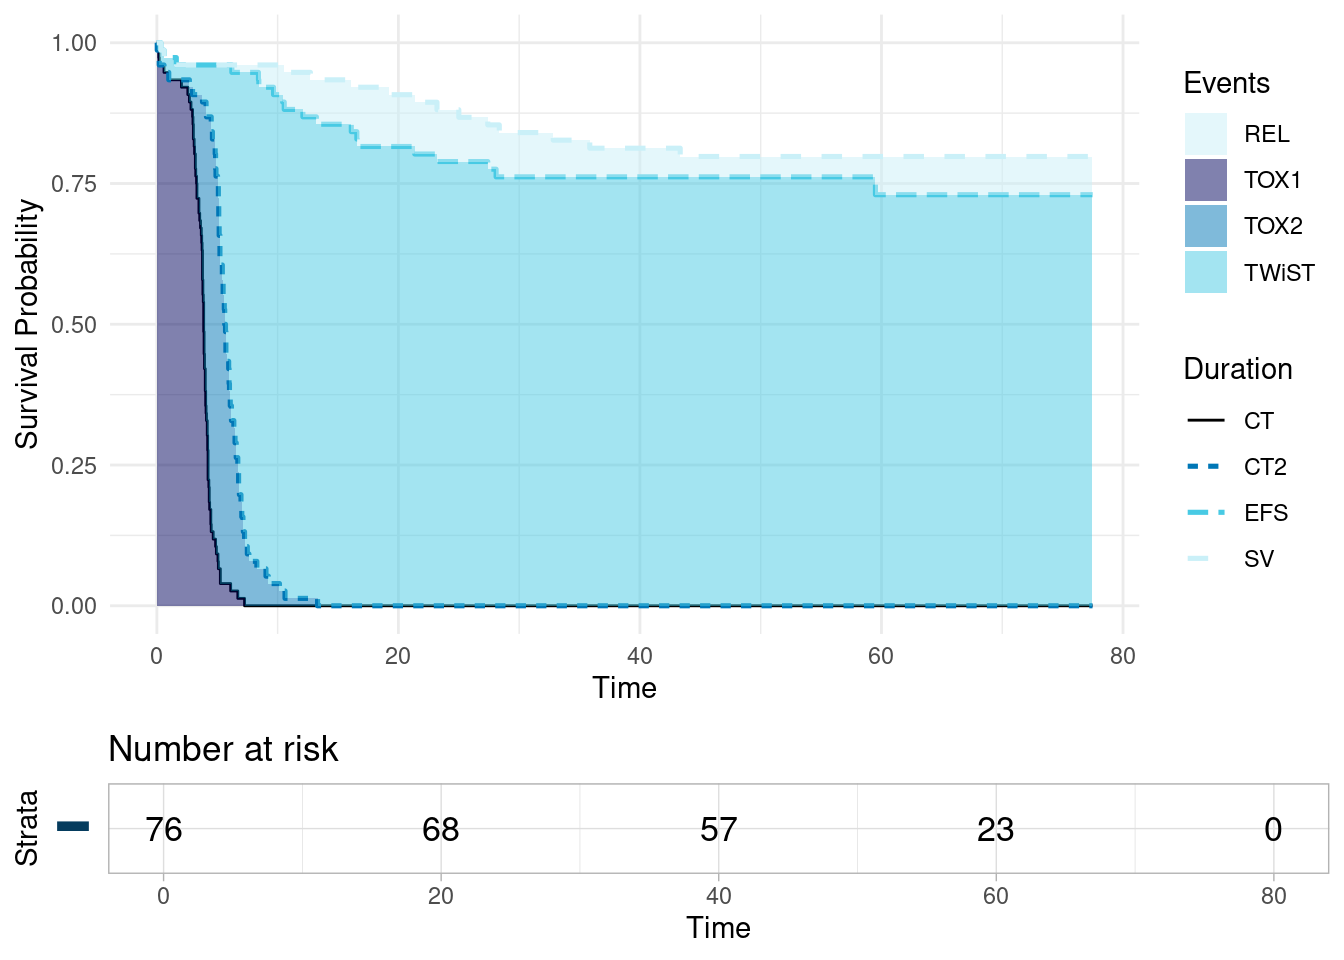
\includegraphics{partition_files/figure-latex/unnamed-chunk-3-1.pdf}

\hypertarget{partition-1}{%
\paragraph{Partition 1}\label{partition-1}}

\begin{Shaded}
\begin{Highlighting}[]
\FunctionTok{library}\NormalTok{(survminer)}
\FunctionTok{library}\NormalTok{(survival)}
\FunctionTok{library}\NormalTok{(gridExtra) }\CommentTok{\# or library(patchwork)}

\CommentTok{\# Assuming ct, sv, and efs are survival objects}
\NormalTok{fit1 }\OtherTok{\textless{}{-}} \FunctionTok{list}\NormalTok{(}\AttributeTok{CT =}\NormalTok{ ct\_A, }\AttributeTok{SV =}\NormalTok{ sv\_A, }\AttributeTok{EFS =}\NormalTok{ efs\_A)}

\CommentTok{\# custom color palette for CT, SV, EFS}
\NormalTok{colors }\OtherTok{\textless{}{-}} \FunctionTok{c}\NormalTok{(}\StringTok{"\#A31621"}\NormalTok{, }\StringTok{"\#053C5E"}\NormalTok{, }\StringTok{"\#F3A712"}\NormalTok{, }\StringTok{"\#1F7A8C"}\NormalTok{, }\StringTok{"\#AFB3F7"}\NormalTok{)}

\CommentTok{\# Step 1: Generate the Combined Survival Plot without a risk table}
\NormalTok{surv1\_A }\OtherTok{\textless{}{-}} \FunctionTok{ggsurvplot\_combine}\NormalTok{(fit1,}
                        \AttributeTok{risk.table =} \ConstantTok{FALSE}\NormalTok{,  }\CommentTok{\# Disable risk table here}
                        \AttributeTok{xlab =} \StringTok{"Time in days"}\NormalTok{,}
                        \AttributeTok{ggtheme =} \FunctionTok{theme\_light}\NormalTok{(),}
                        \AttributeTok{legend.labs =} \FunctionTok{c}\NormalTok{(}\StringTok{"CT"}\NormalTok{,}\StringTok{"SV"}\NormalTok{,}\StringTok{"EFS"}\NormalTok{),}
                        \AttributeTok{palette=}\NormalTok{colors,}
                        \AttributeTok{title=}\StringTok{"Bras A"}\NormalTok{)}

\CommentTok{\# Step 2: Generate a Separate Risk Table for "SV"}
\CommentTok{\# Note: This assumes \textquotesingle{}sv\textquotesingle{} is a fit object from survival analysis.}
\CommentTok{\# If \textquotesingle{}sv\textquotesingle{} is not directly usable, you might need to recreate the survival analysis for SV.}
\NormalTok{sv\_plot\_A }\OtherTok{\textless{}{-}} \FunctionTok{ggsurvplot}\NormalTok{(sv\_A, }\AttributeTok{risk.table =} \ConstantTok{TRUE}\NormalTok{,}
                      \AttributeTok{ggtheme =} \FunctionTok{theme\_light}\NormalTok{(),}
                      \CommentTok{\# tables.theme = theme(}
                      \CommentTok{\#   axis.text.x = element\_blank(),  \# Hide x{-}axis text}
                      \CommentTok{\#   axis.ticks.x = element\_blank(), \# Hide x{-}axis ticks}
                      \CommentTok{\#   axis.title.x = element\_blank()  \# Optionally, hide the x{-}axis title as well}
                      \CommentTok{\# ),}
                      \AttributeTok{risk.table.y.text.col =} \ConstantTok{TRUE}\NormalTok{,}
                      \AttributeTok{risk.table.y.text =} \ConstantTok{FALSE}\NormalTok{,}
                      \AttributeTok{palette =}\NormalTok{ colors[}\DecValTok{2}\NormalTok{])  }\CommentTok{\# Adjust \textquotesingle{}colors[2]\textquotesingle{} as per your color setup}


\CommentTok{\# Step 3: Combine the Plot and the Risk Table Manually}
\CommentTok{\# Option 1: Using gridExtra}
\NormalTok{combined\_plot }\OtherTok{\textless{}{-}} \FunctionTok{grid.arrange}\NormalTok{(surv1\_A}\SpecialCharTok{$}\NormalTok{plot, sv\_plot\_A}\SpecialCharTok{$}\NormalTok{table, }\AttributeTok{ncol =} \DecValTok{1}\NormalTok{,}\AttributeTok{heights =} \FunctionTok{c}\NormalTok{(}\DecValTok{6}\NormalTok{, }\DecValTok{2}\NormalTok{))}
\end{Highlighting}
\end{Shaded}

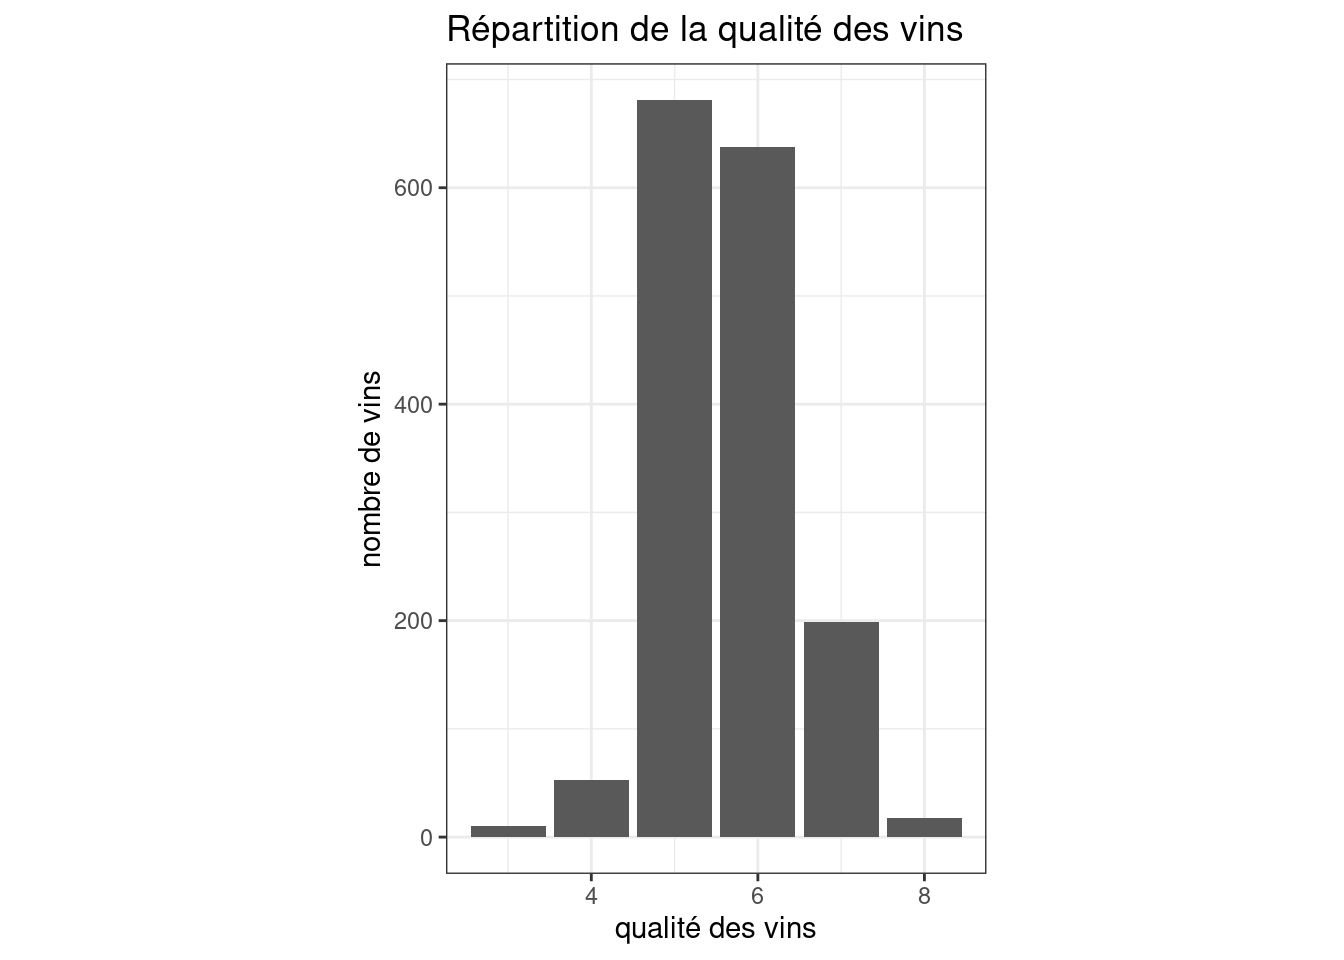
\includegraphics{partition_files/figure-latex/unnamed-chunk-4-1.pdf}

\begin{Shaded}
\begin{Highlighting}[]
\CommentTok{\# Or Option 2: Using patchwork (Uncomment to use)}
\CommentTok{\# combined\_plot \textless{}{-} g$plot / sv\_plot$table}

\CommentTok{\# Print or save the combined plot}
\FunctionTok{print}\NormalTok{(combined\_plot)}
\end{Highlighting}
\end{Shaded}

\begin{verbatim}
## TableGrob (2 x 1) "arrange": 2 grobs
##   z     cells    name           grob
## 1 1 (1-1,1-1) arrange gtable[layout]
## 2 2 (2-2,1-1) arrange gtable[layout]
\end{verbatim}

\hypertarget{partition-2}{%
\paragraph{Partition 2}\label{partition-2}}

\begin{Shaded}
\begin{Highlighting}[]
\FunctionTok{library}\NormalTok{(survminer)}
\FunctionTok{library}\NormalTok{(survival)}
\FunctionTok{library}\NormalTok{(gridExtra) }\CommentTok{\# or library(patchwork)}

\CommentTok{\# Assuming ct, sv, and efs are survival objects}
\NormalTok{fit2 }\OtherTok{\textless{}{-}} \FunctionTok{list}\NormalTok{(}\AttributeTok{CT =}\NormalTok{ ct\_A, }\AttributeTok{SV =}\NormalTok{ sv\_A, }\AttributeTok{EFS =}\NormalTok{ efs\_A, }\AttributeTok{CT2 =}\NormalTok{ ct2\_A)}

\CommentTok{\# custom color palette for CT, SV, EFS}
\NormalTok{colors }\OtherTok{\textless{}{-}} \FunctionTok{c}\NormalTok{(}\StringTok{"\#A31621"}\NormalTok{, }\StringTok{"\#053C5E"}\NormalTok{, }\StringTok{"\#F3A712"}\NormalTok{, }\StringTok{"\#1F7A8C"}\NormalTok{, }\StringTok{"\#AFB3F7"}\NormalTok{)}

\CommentTok{\# Step 1: Generate the Combined Survival Plot without a risk table}
\NormalTok{surv2\_A }\OtherTok{\textless{}{-}} \FunctionTok{ggsurvplot\_combine}\NormalTok{(fit2,}
                        \AttributeTok{risk.table =} \ConstantTok{FALSE}\NormalTok{,  }\CommentTok{\# Disable risk table here}
                        \AttributeTok{xlab =} \StringTok{"Time in days"}\NormalTok{,}
                        \AttributeTok{ggtheme =} \FunctionTok{theme\_light}\NormalTok{(),}
                        \AttributeTok{legend.labs =} \FunctionTok{c}\NormalTok{(}\StringTok{"CT"}\NormalTok{,}\StringTok{"SV"}\NormalTok{,}\StringTok{"EFS"}\NormalTok{,}\StringTok{"CT2"}\NormalTok{),}
                        \AttributeTok{palette=}\NormalTok{colors,}
                        \AttributeTok{title=}\StringTok{"Bras A"}\NormalTok{)}



\CommentTok{\# Step 3: Combine the Plot and the Risk Table Manually}
\CommentTok{\# Option 1: Using gridExtra}
\NormalTok{combined\_plot }\OtherTok{\textless{}{-}} \FunctionTok{grid.arrange}\NormalTok{(surv2\_A}\SpecialCharTok{$}\NormalTok{plot, sv\_plot\_A}\SpecialCharTok{$}\NormalTok{table, }\AttributeTok{ncol =} \DecValTok{1}\NormalTok{,}\AttributeTok{heights =} \FunctionTok{c}\NormalTok{(}\DecValTok{6}\NormalTok{, }\DecValTok{2}\NormalTok{))}
\end{Highlighting}
\end{Shaded}

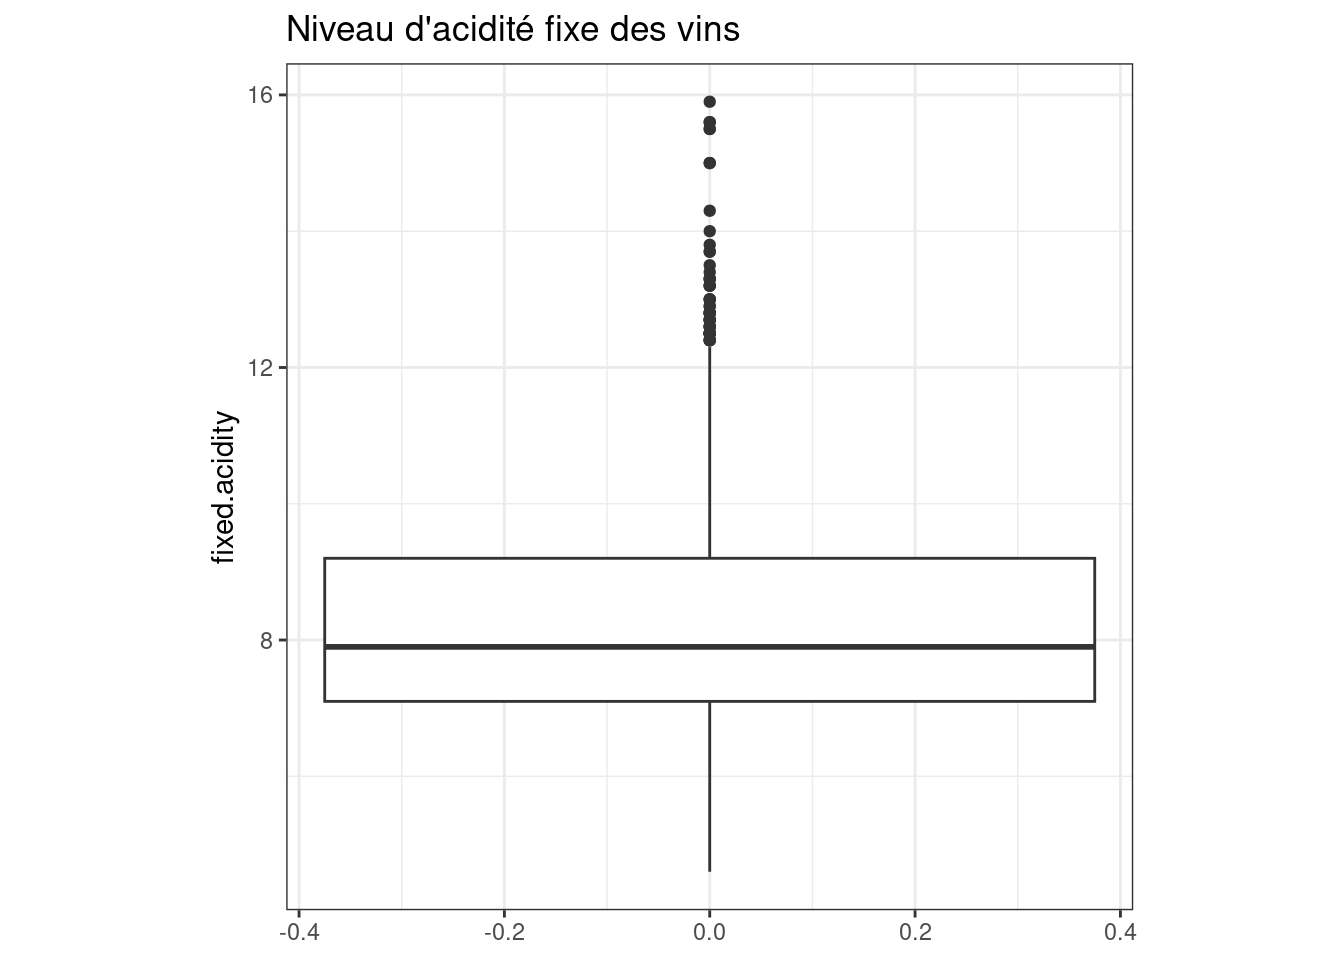
\includegraphics{partition_files/figure-latex/unnamed-chunk-5-1.pdf}

\begin{Shaded}
\begin{Highlighting}[]
\CommentTok{\# Print or save the combined plot}
\FunctionTok{print}\NormalTok{(combined\_plot)}
\end{Highlighting}
\end{Shaded}

\begin{verbatim}
## TableGrob (2 x 1) "arrange": 2 grobs
##   z     cells    name           grob
## 1 1 (1-1,1-1) arrange gtable[layout]
## 2 2 (2-2,1-1) arrange gtable[layout]
\end{verbatim}

\begin{Shaded}
\begin{Highlighting}[]
\CommentTok{\# fit2\textless{}{-}list(CT = ct, CT2 = ct2, SV=sv, EFS=efs)}
\CommentTok{\# library(survminer)}
\CommentTok{\# t\textless{}{-}ggsurvplot\_combine(fit,}
\CommentTok{\#           risk.table = TRUE,                  \# Add risk table}
\CommentTok{\#    xlab = "Time in days",   \# customize X axis label.}
\CommentTok{\#    ggtheme = theme\_light(), \# customize plot and risk table with a therme.}
\CommentTok{\#  risk.table.y.text.col = T, \# colour risk table text annotations.}
\CommentTok{\#   risk.table.y.text = FALSE,}
\CommentTok{\#   legend.labs = c("CT", "CT2","SV","EFS"))}
\CommentTok{\# t}
\end{Highlighting}
\end{Shaded}

\hypertarget{bras-b}{%
\subsubsection{Bras B}\label{bras-b}}

\hypertarget{partition-1-1}{%
\paragraph{Partition 1}\label{partition-1-1}}

\begin{Shaded}
\begin{Highlighting}[]
\FunctionTok{library}\NormalTok{(survminer)}
\FunctionTok{library}\NormalTok{(survival)}
\FunctionTok{library}\NormalTok{(gridExtra) }\CommentTok{\# or library(patchwork)}

\CommentTok{\# Assuming ct, sv, and efs are survival objects}
\NormalTok{fit1 }\OtherTok{\textless{}{-}} \FunctionTok{list}\NormalTok{(}\AttributeTok{CT =}\NormalTok{ ct\_B, }\AttributeTok{SV =}\NormalTok{ sv\_B, }\AttributeTok{EFS =}\NormalTok{ efs\_B)}

\CommentTok{\# custom color palette for CT, SV, EFS}
\NormalTok{colors }\OtherTok{\textless{}{-}} \FunctionTok{c}\NormalTok{(}\StringTok{"\#A31621"}\NormalTok{, }\StringTok{"\#053C5E"}\NormalTok{, }\StringTok{"\#F3A712"}\NormalTok{, }\StringTok{"\#1F7A8C"}\NormalTok{, }\StringTok{"\#AFB3F7"}\NormalTok{)}

\CommentTok{\# Step 1: Generate the Combined Survival Plot without a risk table}
\NormalTok{surv1\_B }\OtherTok{\textless{}{-}} \FunctionTok{ggsurvplot\_combine}\NormalTok{(fit1,}
                        \AttributeTok{risk.table =} \ConstantTok{FALSE}\NormalTok{,  }\CommentTok{\# Disable risk table here}
                        \AttributeTok{xlab =} \StringTok{"Time in days"}\NormalTok{,}
                        \AttributeTok{ggtheme =} \FunctionTok{theme\_light}\NormalTok{(),}
                        \AttributeTok{legend.labs =} \FunctionTok{c}\NormalTok{(}\StringTok{"CT"}\NormalTok{,}\StringTok{"SV"}\NormalTok{,}\StringTok{"EFS"}\NormalTok{),}
                        \AttributeTok{palette=}\NormalTok{colors,}
                        \AttributeTok{title=}\StringTok{"Bras B"}\NormalTok{)}

\CommentTok{\# Step 2: Generate a Separate Risk Table for "SV"}
\CommentTok{\# Note: This assumes \textquotesingle{}sv\textquotesingle{} is a fit object from survival analysis.}
\CommentTok{\# If \textquotesingle{}sv\textquotesingle{} is not directly usable, you might need to recreate the survival analysis for SV.}
\NormalTok{sv\_plot\_B }\OtherTok{\textless{}{-}} \FunctionTok{ggsurvplot}\NormalTok{(sv\_B, }\AttributeTok{risk.table =} \ConstantTok{TRUE}\NormalTok{,}
                      \AttributeTok{ggtheme =} \FunctionTok{theme\_light}\NormalTok{(),}
                      \CommentTok{\# tables.theme = theme(}
                      \CommentTok{\#   axis.text.x = element\_blank(),  \# Hide x{-}axis text}
                      \CommentTok{\#   axis.ticks.x = element\_blank(), \# Hide x{-}axis ticks}
                      \CommentTok{\#   axis.title.x = element\_blank()  \# Optionally, hide the x{-}axis title as well}
                      \CommentTok{\# ),}
                      \AttributeTok{risk.table.y.text.col =} \ConstantTok{TRUE}\NormalTok{,}
                      \AttributeTok{risk.table.y.text =} \ConstantTok{FALSE}\NormalTok{,}
                      \AttributeTok{palette =}\NormalTok{ colors[}\DecValTok{2}\NormalTok{])  }\CommentTok{\# Adjust \textquotesingle{}colors[2]\textquotesingle{} as per your color setup}


\CommentTok{\# Step 3: Combine the Plot and the Risk Table Manually}
\CommentTok{\# Option 1: Using gridExtra}
\NormalTok{combined\_plot }\OtherTok{\textless{}{-}} \FunctionTok{grid.arrange}\NormalTok{(surv1\_B}\SpecialCharTok{$}\NormalTok{plot, sv\_plot\_B}\SpecialCharTok{$}\NormalTok{table, }\AttributeTok{ncol =} \DecValTok{1}\NormalTok{,}\AttributeTok{heights =} \FunctionTok{c}\NormalTok{(}\DecValTok{6}\NormalTok{, }\DecValTok{2}\NormalTok{))}
\end{Highlighting}
\end{Shaded}

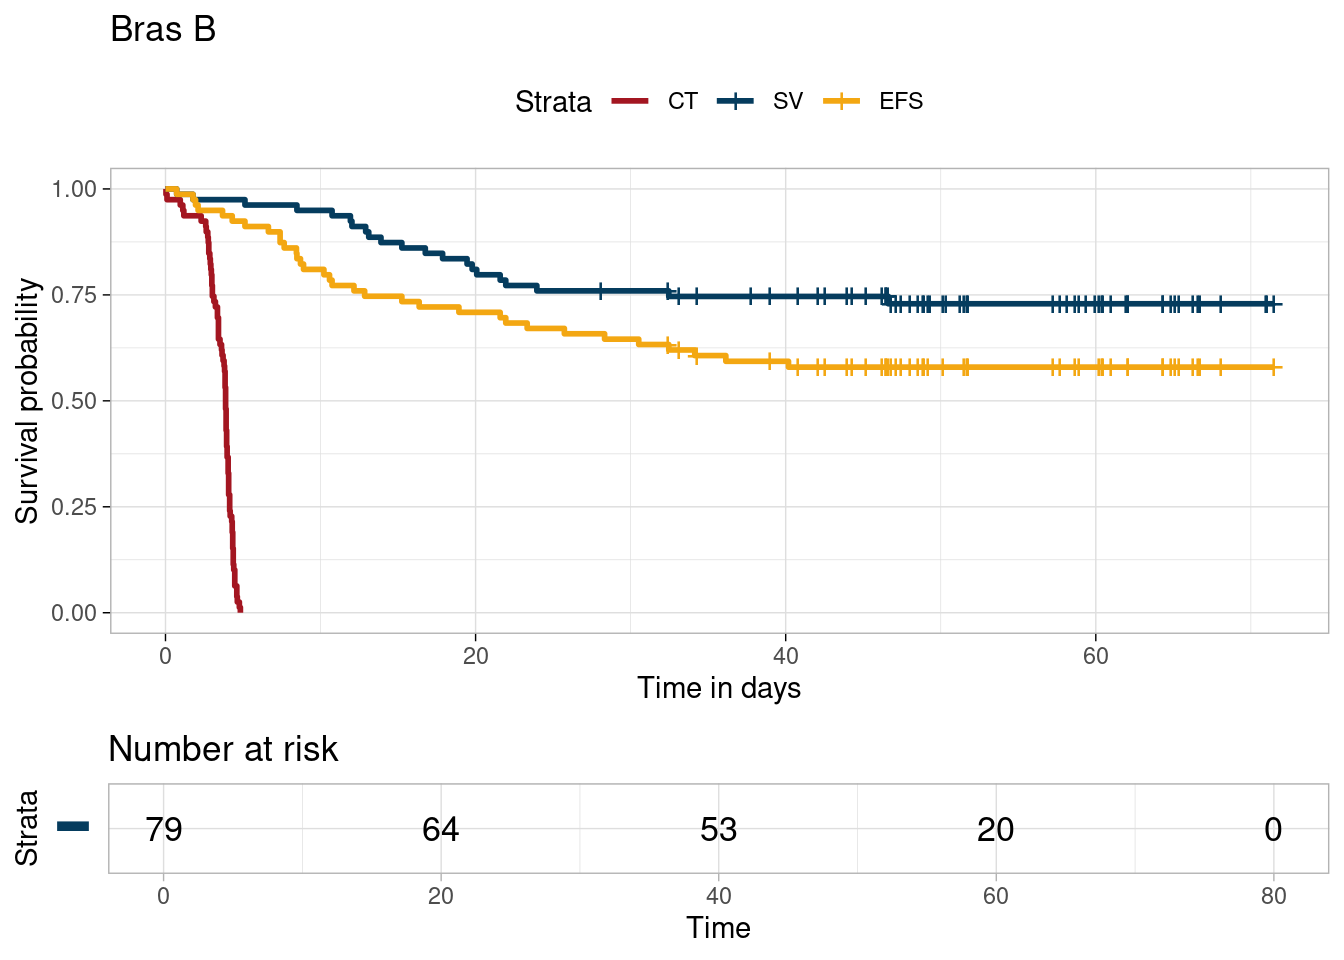
\includegraphics{partition_files/figure-latex/unnamed-chunk-7-1.pdf}

\begin{Shaded}
\begin{Highlighting}[]
\CommentTok{\# Or Option 2: Using patchwork (Uncomment to use)}
\CommentTok{\# combined\_plot \textless{}{-} g$plot / sv\_plot$table}

\CommentTok{\# Print or save the combined plot}
\FunctionTok{print}\NormalTok{(combined\_plot)}
\end{Highlighting}
\end{Shaded}

\begin{verbatim}
## TableGrob (2 x 1) "arrange": 2 grobs
##   z     cells    name           grob
## 1 1 (1-1,1-1) arrange gtable[layout]
## 2 2 (2-2,1-1) arrange gtable[layout]
\end{verbatim}

\hypertarget{partition-2-1}{%
\paragraph{Partition 2}\label{partition-2-1}}

\begin{Shaded}
\begin{Highlighting}[]
\FunctionTok{library}\NormalTok{(survminer)}
\FunctionTok{library}\NormalTok{(survival)}
\FunctionTok{library}\NormalTok{(gridExtra) }\CommentTok{\# or library(patchwork)}

\CommentTok{\# Assuming ct, sv, and efs are survival objects}
\NormalTok{fit2 }\OtherTok{\textless{}{-}} \FunctionTok{list}\NormalTok{(}\AttributeTok{CT =}\NormalTok{ ct\_B, }\AttributeTok{SV =}\NormalTok{ sv\_B, }\AttributeTok{EFS =}\NormalTok{ efs\_B, }\AttributeTok{CT2 =}\NormalTok{ ct2\_B)}

\CommentTok{\# custom color palette for CT, SV, EFS}
\NormalTok{colors }\OtherTok{\textless{}{-}} \FunctionTok{c}\NormalTok{(}\StringTok{"\#A31621"}\NormalTok{, }\StringTok{"\#053C5E"}\NormalTok{, }\StringTok{"\#F3A712"}\NormalTok{, }\StringTok{"\#1F7A8C"}\NormalTok{, }\StringTok{"\#AFB3F7"}\NormalTok{)}

\CommentTok{\# Step 1: Generate the Combined Survival Plot without a risk table}
\NormalTok{surv2\_B }\OtherTok{\textless{}{-}} \FunctionTok{ggsurvplot\_combine}\NormalTok{(fit2,}
                        \AttributeTok{risk.table =} \ConstantTok{FALSE}\NormalTok{,  }\CommentTok{\# Disable risk table here}
                        \AttributeTok{xlab =} \StringTok{"Time in days"}\NormalTok{,}
                        \AttributeTok{ggtheme =} \FunctionTok{theme\_light}\NormalTok{(),}
                        \AttributeTok{legend.labs =} \FunctionTok{c}\NormalTok{(}\StringTok{"CT"}\NormalTok{,}\StringTok{"SV"}\NormalTok{,}\StringTok{"EFS"}\NormalTok{,}\StringTok{"CT2"}\NormalTok{),}
                        \AttributeTok{palette=}\NormalTok{colors,}
                        \AttributeTok{title=}\StringTok{"Bras B"}\NormalTok{)}



\CommentTok{\# Step 3: Combine the Plot and the Risk Table Manually}
\CommentTok{\# Option 1: Using gridExtra}
\NormalTok{combined\_plot }\OtherTok{\textless{}{-}} \FunctionTok{grid.arrange}\NormalTok{(surv2\_B}\SpecialCharTok{$}\NormalTok{plot, sv\_plot\_B}\SpecialCharTok{$}\NormalTok{table, }\AttributeTok{ncol =} \DecValTok{1}\NormalTok{,}\AttributeTok{heights =} \FunctionTok{c}\NormalTok{(}\DecValTok{6}\NormalTok{, }\DecValTok{2}\NormalTok{))}
\end{Highlighting}
\end{Shaded}

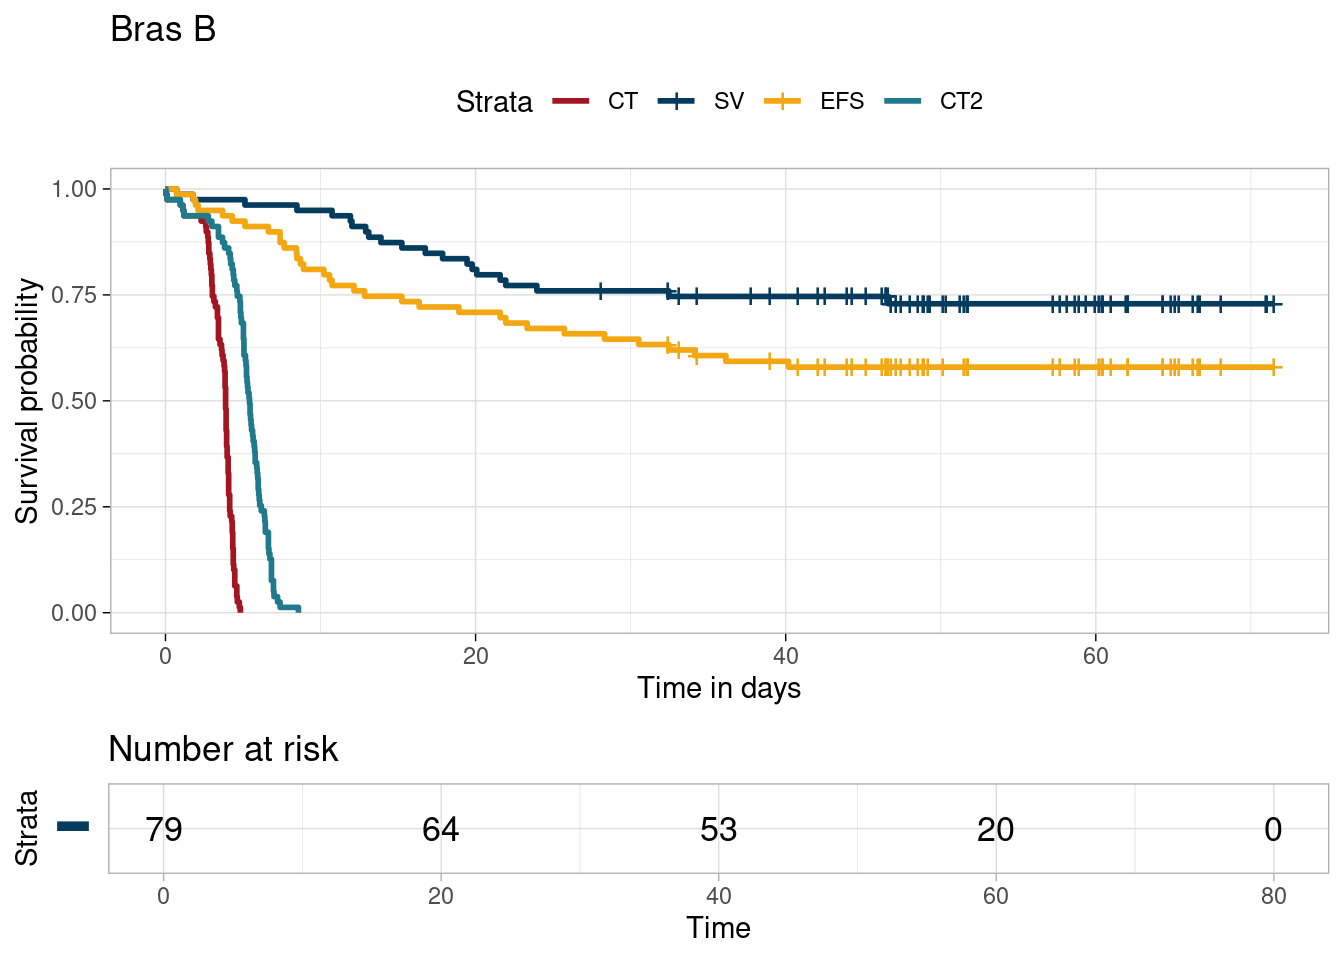
\includegraphics{partition_files/figure-latex/unnamed-chunk-8-1.pdf}

\begin{Shaded}
\begin{Highlighting}[]
\CommentTok{\# Print or save the combined plot}
\FunctionTok{print}\NormalTok{(combined\_plot)}
\end{Highlighting}
\end{Shaded}

\begin{verbatim}
## TableGrob (2 x 1) "arrange": 2 grobs
##   z     cells    name           grob
## 1 1 (1-1,1-1) arrange gtable[layout]
## 2 2 (2-2,1-1) arrange gtable[layout]
\end{verbatim}

\hypertarget{rmst}{%
\section{RMST}\label{rmst}}

\hypertarget{computing-rmst-for-each-arm}{%
\subsection{Computing rmst for each
arm}\label{computing-rmst-for-each-arm}}

\begin{Shaded}
\begin{Highlighting}[]
\CommentTok{\# Charger les packages nécessaires}
\FunctionTok{library}\NormalTok{(survival)}
\FunctionTok{library}\NormalTok{(survRM2) }\CommentTok{\# Assurez{-}vous que le package rmst2 est installé pour accéder à cette fonction}
\FunctionTok{library}\NormalTok{(boot)}

\DocumentationTok{\#\#\# 0 = Int arm A, 1 = Light arm B}
\NormalTok{t\_censure }\OtherTok{\textless{}{-}} \DecValTok{60}\CommentTok{\#min(64.3285421,60.9774127) \# 20\% de censure}

\CommentTok{\# For ct\_rmst}
\NormalTok{ct\_rmst}\OtherTok{\textless{}{-}}\FunctionTok{rmst2}\NormalTok{(qaly}\SpecialCharTok{$}\NormalTok{delfinct, qaly}\SpecialCharTok{$}\NormalTok{finct, }\FunctionTok{as.factor}\NormalTok{(}\FunctionTok{as.numeric}\NormalTok{(qaly}\SpecialCharTok{$}\NormalTok{R1)}\SpecialCharTok{{-}}\DecValTok{1}\NormalTok{), }\AttributeTok{covariates =} \ConstantTok{NULL}\NormalTok{, }\AttributeTok{alpha =} \FloatTok{0.05}\NormalTok{)}

\NormalTok{ct\_rmstB}\OtherTok{\textless{}{-}}\NormalTok{ct\_rmst}\SpecialCharTok{$}\NormalTok{RMST.arm1}\SpecialCharTok{$}\NormalTok{rmst[}\DecValTok{1}\NormalTok{]}
\NormalTok{ct\_rmstA}\OtherTok{\textless{}{-}}\NormalTok{ct\_rmst}\SpecialCharTok{$}\NormalTok{RMST.arm0}\SpecialCharTok{$}\NormalTok{rmst[}\DecValTok{1}\NormalTok{]}

\CommentTok{\# For ct2\_rmst}
\NormalTok{ct2\_rmst}\OtherTok{\textless{}{-}}\FunctionTok{rmst2}\NormalTok{(qaly}\SpecialCharTok{$}\NormalTok{delfinct2, qaly}\SpecialCharTok{$}\NormalTok{finct2, }\FunctionTok{as.factor}\NormalTok{(}\FunctionTok{as.numeric}\NormalTok{(qaly}\SpecialCharTok{$}\NormalTok{R1)}\SpecialCharTok{{-}}\DecValTok{1}\NormalTok{), }\AttributeTok{covariates =} \ConstantTok{NULL}\NormalTok{, }\AttributeTok{alpha =} \FloatTok{0.05}\NormalTok{)}
\NormalTok{ct2\_rmstB }\OtherTok{\textless{}{-}}\NormalTok{ ct2\_rmst}\SpecialCharTok{$}\NormalTok{RMST.arm1}\SpecialCharTok{$}\NormalTok{rmst[}\DecValTok{1}\NormalTok{]  }\CommentTok{\# Assuming arm1 corresponds to arm B}
\NormalTok{ct2\_rmstA }\OtherTok{\textless{}{-}}\NormalTok{ ct2\_rmst}\SpecialCharTok{$}\NormalTok{RMST.arm0}\SpecialCharTok{$}\NormalTok{rmst[}\DecValTok{1}\NormalTok{]  }\CommentTok{\# Assuming arm0 corresponds to arm A}

\CommentTok{\# For sv\_rmst}
\NormalTok{sv\_rmst}\OtherTok{\textless{}{-}}\FunctionTok{rmst2}\NormalTok{(qaly}\SpecialCharTok{$}\NormalTok{suivi, }\FunctionTok{as.numeric}\NormalTok{(}\FunctionTok{as.character}\NormalTok{(qaly}\SpecialCharTok{$}\NormalTok{dc)), }\FunctionTok{as.factor}\NormalTok{(}\FunctionTok{as.numeric}\NormalTok{(qaly}\SpecialCharTok{$}\NormalTok{R1)}\SpecialCharTok{{-}}\DecValTok{1}\NormalTok{), }\AttributeTok{tau =}\NormalTok{ t\_censure, }\AttributeTok{covariates =} \ConstantTok{NULL}\NormalTok{, }\AttributeTok{alpha =} \FloatTok{0.05}\NormalTok{)}
\NormalTok{sv\_rmstB }\OtherTok{\textless{}{-}}\NormalTok{ sv\_rmst}\SpecialCharTok{$}\NormalTok{RMST.arm1}\SpecialCharTok{$}\NormalTok{rmst[}\DecValTok{1}\NormalTok{]}
\NormalTok{sv\_rmstA }\OtherTok{\textless{}{-}}\NormalTok{ sv\_rmst}\SpecialCharTok{$}\NormalTok{RMST.arm0}\SpecialCharTok{$}\NormalTok{rmst[}\DecValTok{1}\NormalTok{]}

\CommentTok{\# For efs\_rmst}
\NormalTok{efs\_rmst}\OtherTok{\textless{}{-}}\FunctionTok{rmst2}\NormalTok{(qaly}\SpecialCharTok{$}\NormalTok{delpfs, }\FunctionTok{as.numeric}\NormalTok{(}\FunctionTok{as.character}\NormalTok{(qaly}\SpecialCharTok{$}\NormalTok{pfs)), }\FunctionTok{as.factor}\NormalTok{(}\FunctionTok{as.numeric}\NormalTok{(qaly}\SpecialCharTok{$}\NormalTok{R1)}\SpecialCharTok{{-}}\DecValTok{1}\NormalTok{), }\AttributeTok{tau =}\NormalTok{ t\_censure, }\AttributeTok{covariates =} \ConstantTok{NULL}\NormalTok{, }\AttributeTok{alpha =} \FloatTok{0.05}\NormalTok{)}
\NormalTok{efs\_rmstB }\OtherTok{\textless{}{-}}\NormalTok{ efs\_rmst}\SpecialCharTok{$}\NormalTok{RMST.arm1}\SpecialCharTok{$}\NormalTok{rmst[}\DecValTok{1}\NormalTok{]}
\NormalTok{efs\_rmstA }\OtherTok{\textless{}{-}}\NormalTok{ efs\_rmst}\SpecialCharTok{$}\NormalTok{RMST.arm0}\SpecialCharTok{$}\NormalTok{rmst[}\DecValTok{1}\NormalTok{]}

\CommentTok{\# Calculer TOX, TWiST, et REL en utilisant les RMST calculés}
\NormalTok{tox1\_A }\OtherTok{=}\NormalTok{ ct\_rmstA}
\NormalTok{tox2\_A }\OtherTok{=}\NormalTok{ ct2\_rmstA}
\NormalTok{twist1\_A }\OtherTok{=}\NormalTok{ efs\_rmstA }\SpecialCharTok{{-}}\NormalTok{ ct\_rmstA}
\NormalTok{twist2\_A}\OtherTok{=}\NormalTok{ efs\_rmstA }\SpecialCharTok{{-}}\NormalTok{ ct2\_rmstA}
\NormalTok{rel\_A }\OtherTok{=}\NormalTok{ sv\_rmstA }\SpecialCharTok{{-}}\NormalTok{ efs\_rmstA}


\CommentTok{\# Calculer TOX, TWiST, et REL en utilisant les RMST calculés}
\NormalTok{tox1\_B }\OtherTok{=}\NormalTok{ ct\_rmstB}
\NormalTok{tox2\_B }\OtherTok{=}\NormalTok{ ct2\_rmstB}
\NormalTok{twist1\_B }\OtherTok{=}\NormalTok{ efs\_rmstB }\SpecialCharTok{{-}}\NormalTok{ ct\_rmstB}
\NormalTok{twist2\_B}\OtherTok{=}\NormalTok{ efs\_rmstB }\SpecialCharTok{{-}}\NormalTok{ ct2\_rmstB}
\NormalTok{rel\_B }\OtherTok{=}\NormalTok{ sv\_rmstB }\SpecialCharTok{{-}}\NormalTok{ efs\_rmstB}
\end{Highlighting}
\end{Shaded}

\hypertarget{boostrapping}{%
\paragraph{Boostrapping}\label{boostrapping}}

\hypertarget{toxtwistrel-their-differences-between-group}{%
\subparagraph{TOX/TWISt/REL \& their differences between
group}\label{toxtwistrel-their-differences-between-group}}

\begin{Shaded}
\begin{Highlighting}[]
\CommentTok{\# Fonction pour calculer les RMST sur un échantillon bootstrapé}

\NormalTok{calculate\_rmst }\OtherTok{\textless{}{-}} \ControlFlowTok{function}\NormalTok{(data, indices, uTWiST, uTOX, uREL, t\_censure) \{}
\NormalTok{  sampled\_data }\OtherTok{\textless{}{-}}\NormalTok{ data[indices, ]}
  
  \CommentTok{\# Calculer les RMST pour chaque bras et chaque étape}
\NormalTok{  ct\_rmst }\OtherTok{\textless{}{-}} \FunctionTok{rmst2}\NormalTok{(sampled\_data}\SpecialCharTok{$}\NormalTok{delfinct, sampled\_data}\SpecialCharTok{$}\NormalTok{finct, }\FunctionTok{as.factor}\NormalTok{(}\FunctionTok{as.numeric}\NormalTok{(sampled\_data}\SpecialCharTok{$}\NormalTok{R1)}\SpecialCharTok{{-}}\DecValTok{1}\NormalTok{), }\AttributeTok{covariates =} \ConstantTok{NULL}\NormalTok{, }\AttributeTok{alpha =} \FloatTok{0.05}\NormalTok{)}
\NormalTok{  ct\_rmstB }\OtherTok{\textless{}{-}}\NormalTok{ ct\_rmst}\SpecialCharTok{$}\NormalTok{RMST.arm1}\SpecialCharTok{$}\NormalTok{rmst[}\DecValTok{1}\NormalTok{]}
\NormalTok{  ct\_rmstA }\OtherTok{\textless{}{-}}\NormalTok{ ct\_rmst}\SpecialCharTok{$}\NormalTok{RMST.arm0}\SpecialCharTok{$}\NormalTok{rmst[}\DecValTok{1}\NormalTok{]}
  
\NormalTok{  ct2\_rmst }\OtherTok{\textless{}{-}} \FunctionTok{rmst2}\NormalTok{(sampled\_data}\SpecialCharTok{$}\NormalTok{delfinct2, sampled\_data}\SpecialCharTok{$}\NormalTok{finct2, }\FunctionTok{as.factor}\NormalTok{(}\FunctionTok{as.numeric}\NormalTok{(sampled\_data}\SpecialCharTok{$}\NormalTok{R1)}\SpecialCharTok{{-}}\DecValTok{1}\NormalTok{), }\AttributeTok{covariates =} \ConstantTok{NULL}\NormalTok{, }\AttributeTok{alpha =} \FloatTok{0.05}\NormalTok{)}
\NormalTok{  ct2\_rmstB }\OtherTok{\textless{}{-}}\NormalTok{ ct2\_rmst}\SpecialCharTok{$}\NormalTok{RMST.arm1}\SpecialCharTok{$}\NormalTok{rmst[}\DecValTok{1}\NormalTok{]}
\NormalTok{  ct2\_rmstA }\OtherTok{\textless{}{-}}\NormalTok{ ct2\_rmst}\SpecialCharTok{$}\NormalTok{RMST.arm0}\SpecialCharTok{$}\NormalTok{rmst[}\DecValTok{1}\NormalTok{]}
  
\NormalTok{  sv\_rmst }\OtherTok{\textless{}{-}} \FunctionTok{rmst2}\NormalTok{(sampled\_data}\SpecialCharTok{$}\NormalTok{suivi, }\FunctionTok{as.numeric}\NormalTok{(}\FunctionTok{as.character}\NormalTok{(sampled\_data}\SpecialCharTok{$}\NormalTok{dc)), }\FunctionTok{as.factor}\NormalTok{(}\FunctionTok{as.numeric}\NormalTok{(sampled\_data}\SpecialCharTok{$}\NormalTok{R1)}\SpecialCharTok{{-}}\DecValTok{1}\NormalTok{), }\AttributeTok{tau =}\NormalTok{ t\_censure, }\AttributeTok{covariates =} \ConstantTok{NULL}\NormalTok{, }\AttributeTok{alpha =} \FloatTok{0.05}\NormalTok{)}
\NormalTok{  sv\_rmstB }\OtherTok{\textless{}{-}}\NormalTok{ sv\_rmst}\SpecialCharTok{$}\NormalTok{RMST.arm1}\SpecialCharTok{$}\NormalTok{rmst[}\DecValTok{1}\NormalTok{]}
\NormalTok{  sv\_rmstA }\OtherTok{\textless{}{-}}\NormalTok{ sv\_rmst}\SpecialCharTok{$}\NormalTok{RMST.arm0}\SpecialCharTok{$}\NormalTok{rmst[}\DecValTok{1}\NormalTok{]}
  
\NormalTok{  efs\_rmst }\OtherTok{\textless{}{-}} \FunctionTok{rmst2}\NormalTok{(sampled\_data}\SpecialCharTok{$}\NormalTok{delpfs, }\FunctionTok{as.numeric}\NormalTok{(}\FunctionTok{as.character}\NormalTok{(sampled\_data}\SpecialCharTok{$}\NormalTok{pfs)), }\FunctionTok{as.factor}\NormalTok{(}\FunctionTok{as.numeric}\NormalTok{(sampled\_data}\SpecialCharTok{$}\NormalTok{R1)}\SpecialCharTok{{-}}\DecValTok{1}\NormalTok{), }\AttributeTok{tau =}\NormalTok{ t\_censure, }\AttributeTok{covariates =} \ConstantTok{NULL}\NormalTok{, }\AttributeTok{alpha =} \FloatTok{0.05}\NormalTok{)}
\NormalTok{  efs\_rmstB }\OtherTok{\textless{}{-}}\NormalTok{ efs\_rmst}\SpecialCharTok{$}\NormalTok{RMST.arm1}\SpecialCharTok{$}\NormalTok{rmst[}\DecValTok{1}\NormalTok{]}
\NormalTok{  efs\_rmstA }\OtherTok{\textless{}{-}}\NormalTok{ efs\_rmst}\SpecialCharTok{$}\NormalTok{RMST.arm0}\SpecialCharTok{$}\NormalTok{rmst[}\DecValTok{1}\NormalTok{]}
  
  \CommentTok{\# Calculer les tox, twists et rels pour chaque bras et chaque étape}
\NormalTok{  tox1\_A }\OtherTok{\textless{}{-}}\NormalTok{ ct\_rmstA}
\NormalTok{  tox2\_A }\OtherTok{\textless{}{-}}\NormalTok{ ct2\_rmstA}
\NormalTok{  twist1\_A }\OtherTok{\textless{}{-}}\NormalTok{ efs\_rmstA }\SpecialCharTok{{-}}\NormalTok{ ct\_rmstA}
\NormalTok{  twist2\_A }\OtherTok{\textless{}{-}}\NormalTok{ efs\_rmstA }\SpecialCharTok{{-}}\NormalTok{ ct2\_rmstA}
\NormalTok{  rel\_A }\OtherTok{\textless{}{-}}\NormalTok{ sv\_rmstA }\SpecialCharTok{{-}}\NormalTok{ efs\_rmstA}
  
\NormalTok{  tox1\_B }\OtherTok{\textless{}{-}}\NormalTok{ ct\_rmstB}
\NormalTok{  tox2\_B }\OtherTok{\textless{}{-}}\NormalTok{ ct2\_rmstB}
\NormalTok{  twist1\_B }\OtherTok{\textless{}{-}}\NormalTok{ efs\_rmstB }\SpecialCharTok{{-}}\NormalTok{ ct\_rmstB}
\NormalTok{  twist2\_B }\OtherTok{\textless{}{-}}\NormalTok{ efs\_rmstB }\SpecialCharTok{{-}}\NormalTok{ ct2\_rmstB}
\NormalTok{  rel\_B }\OtherTok{\textless{}{-}}\NormalTok{ sv\_rmstB }\SpecialCharTok{{-}}\NormalTok{ efs\_rmstB}
  
  \CommentTok{\# Calculer les différences entre les bras}
\NormalTok{  tox1\_diff }\OtherTok{\textless{}{-}}\NormalTok{ tox1\_A }\SpecialCharTok{{-}}\NormalTok{ tox1\_B}
\NormalTok{  tox2\_diff }\OtherTok{\textless{}{-}}\NormalTok{ tox2\_A }\SpecialCharTok{{-}}\NormalTok{ tox2\_B}
\NormalTok{  twist1\_diff }\OtherTok{\textless{}{-}}\NormalTok{ twist1\_A }\SpecialCharTok{{-}}\NormalTok{ twist1\_B}
\NormalTok{  twist2\_diff }\OtherTok{\textless{}{-}}\NormalTok{ twist2\_A }\SpecialCharTok{{-}}\NormalTok{ twist2\_B}
\NormalTok{  rel\_diff }\OtherTok{\textless{}{-}}\NormalTok{ rel\_A }\SpecialCharTok{{-}}\NormalTok{ rel\_B}
  
  \CommentTok{\# Calculer QTWiST pour chaque partition}
\NormalTok{  q\_twist1\_A }\OtherTok{\textless{}{-}}\NormalTok{ (uTOX }\SpecialCharTok{*}\NormalTok{ tox1\_A) }\SpecialCharTok{+}\NormalTok{ (uTWiST }\SpecialCharTok{*}\NormalTok{ twist1\_A) }\SpecialCharTok{+}\NormalTok{ (uREL }\SpecialCharTok{*}\NormalTok{ rel\_A)}
\NormalTok{  q\_twist1\_B }\OtherTok{\textless{}{-}}\NormalTok{ (uTOX }\SpecialCharTok{*}\NormalTok{ tox1\_B) }\SpecialCharTok{+}\NormalTok{ (uTWiST }\SpecialCharTok{*}\NormalTok{ twist1\_B) }\SpecialCharTok{+}\NormalTok{ (uREL }\SpecialCharTok{*}\NormalTok{ rel\_B)}
\NormalTok{  q\_twist1\_diff }\OtherTok{\textless{}{-}}\NormalTok{ q\_twist1\_A }\SpecialCharTok{{-}}\NormalTok{ q\_twist1\_B}
  
\NormalTok{  q\_twist2\_A }\OtherTok{\textless{}{-}}\NormalTok{ (uTOX }\SpecialCharTok{*}\NormalTok{ (tox1\_A }\SpecialCharTok{+}\NormalTok{ tox2\_A)) }\SpecialCharTok{+}\NormalTok{ (uTWiST }\SpecialCharTok{*}\NormalTok{ (twist1\_A }\SpecialCharTok{+}\NormalTok{ twist2\_A)) }\SpecialCharTok{+}\NormalTok{ (uREL }\SpecialCharTok{*}\NormalTok{ rel\_A)}
\NormalTok{  q\_twist2\_B }\OtherTok{\textless{}{-}}\NormalTok{ (uTOX }\SpecialCharTok{*}\NormalTok{ (tox1\_B }\SpecialCharTok{+}\NormalTok{ tox2\_B)) }\SpecialCharTok{+}\NormalTok{ (uTWiST }\SpecialCharTok{*}\NormalTok{ (twist1\_B }\SpecialCharTok{+}\NormalTok{ twist2\_B)) }\SpecialCharTok{+}\NormalTok{ (uREL }\SpecialCharTok{*}\NormalTok{ rel\_A)}
\NormalTok{  q\_twist2\_diff }\OtherTok{\textless{}{-}}\NormalTok{ q\_twist2\_A }\SpecialCharTok{{-}}\NormalTok{ q\_twist2\_B}
  
  \CommentTok{\# Retourner les résultats}
  \FunctionTok{return}\NormalTok{(}\FunctionTok{c}\NormalTok{(}\StringTok{"TOX1 A"} \OtherTok{=}\NormalTok{ tox1\_A, }\StringTok{"TOX2 A"} \OtherTok{=}\NormalTok{ tox2\_A, }\StringTok{"TWiST1 A"} \OtherTok{=}\NormalTok{ twist1\_A, }\StringTok{"TWiST2 A"} \OtherTok{=}\NormalTok{ twist2\_A, }\StringTok{"REL A"} \OtherTok{=}\NormalTok{ rel\_A, }
            \StringTok{"TOX1 B"} \OtherTok{=}\NormalTok{ tox1\_B, }\StringTok{"TOX2 B"} \OtherTok{=}\NormalTok{ tox2\_B, }\StringTok{"TWiST1 B"} \OtherTok{=}\NormalTok{ twist1\_B, }\StringTok{"TWiST2 B"} \OtherTok{=}\NormalTok{ twist2\_B, }\StringTok{"REL B"} \OtherTok{=}\NormalTok{ rel\_B, }
            \StringTok{"TOX1diff"} \OtherTok{=}\NormalTok{ tox1\_diff, }\StringTok{"TOX2 diff"} \OtherTok{=}\NormalTok{ tox2\_diff, }\StringTok{"TWiST1 diff"} \OtherTok{=}\NormalTok{ twist1\_diff, }\StringTok{"twist2\_diff"} \OtherTok{=}\NormalTok{ twist2\_diff, }
            \StringTok{"REL diff"} \OtherTok{=}\NormalTok{ rel\_diff,}\StringTok{"q\_TWiST1 A"} \OtherTok{=}\NormalTok{ q\_twist1\_A, }\StringTok{"q\_TWiST1 B"} \OtherTok{=}\NormalTok{ q\_twist1\_B, }\StringTok{"q\_TWiST1 diff"} \OtherTok{=}\NormalTok{ q\_twist1\_diff, }
            \StringTok{"q\_TWiST2 A"} \OtherTok{=}\NormalTok{ q\_twist2\_A, }\StringTok{"q\_TWiST2 B"} \OtherTok{=}\NormalTok{ q\_twist2\_B, }\StringTok{"q\_TWiST2 diff"} \OtherTok{=}\NormalTok{ q\_twist2\_diff))\}}

\CommentTok{\# Appliquer le bootstrap sur le dataset \textquotesingle{}qaly\textquotesingle{}}
\NormalTok{t\_censure }\OtherTok{\textless{}{-}} \FunctionTok{min}\NormalTok{(}\FloatTok{64.3285421}\NormalTok{, }\FloatTok{60.9774127}\NormalTok{) }\CommentTok{\# 20\% de censure}
\NormalTok{qaly\_cens}\OtherTok{\textless{}{-}}\NormalTok{qaly }\SpecialCharTok{\%\textgreater{}\%} \FunctionTok{select}\NormalTok{(delfinct, finct, delfinct2, finct2, suivi, dc, delpfs, pfs, R1)}
\NormalTok{bootstrap\_results1 }\OtherTok{\textless{}{-}} \FunctionTok{censboot}\NormalTok{(qaly\_cens, calculate\_rmst, }\AttributeTok{R =} \DecValTok{1000}\NormalTok{, }\AttributeTok{uTWiST =} \DecValTok{1}\NormalTok{, }\AttributeTok{uTOX =} \FloatTok{0.5}\NormalTok{, }\AttributeTok{uREL =} \FloatTok{0.5}\NormalTok{, }\AttributeTok{t\_censure =}\NormalTok{ t\_censure)}

\NormalTok{boot\_summary}\OtherTok{\textless{}{-}}\FunctionTok{summary}\NormalTok{(bootstrap\_results1) }\SpecialCharTok{\%\textgreater{}\%} \FunctionTok{as.data.frame}\NormalTok{() }
\FunctionTok{rownames}\NormalTok{(boot\_summary) }\OtherTok{\textless{}{-}} \FunctionTok{names}\NormalTok{(bootstrap\_results1}\SpecialCharTok{$}\NormalTok{t0)}
\end{Highlighting}
\end{Shaded}

\hypertarget{threshold-analysis-for-q-twist-diff-with-computed-var-cov}{%
\subsubsection{Threshold analysis for Q-TWIST diff with computed
var-cov}\label{threshold-analysis-for-q-twist-diff-with-computed-var-cov}}

\begin{Shaded}
\begin{Highlighting}[]
\NormalTok{resultsboot}\OtherTok{\textless{}{-}}\FunctionTok{as.data.frame}\NormalTok{(bootstrap\_results1}\SpecialCharTok{$}\NormalTok{t) }\SpecialCharTok{\%\textgreater{}\%}
  \FunctionTok{select}\NormalTok{(}\StringTok{"V1"}\NormalTok{, }\StringTok{"V3"}\NormalTok{, }\StringTok{"V5"}\NormalTok{, }\StringTok{"V6"}\NormalTok{, }\StringTok{"V8"}\NormalTok{, }\StringTok{"V10"}\NormalTok{,}\StringTok{"V11"}\NormalTok{,}\StringTok{"V13"}\NormalTok{,}\StringTok{"V15"}\NormalTok{) }\SpecialCharTok{\%\textgreater{}\%}
  \FunctionTok{rename}\NormalTok{(}\AttributeTok{toxA =} \StringTok{"V1"}\NormalTok{, }\AttributeTok{twistA =} \StringTok{"V3"}\NormalTok{, }\AttributeTok{relA =} \StringTok{"V5"}\NormalTok{, }\AttributeTok{toxB =} \StringTok{"V6"}\NormalTok{, }\AttributeTok{twistB =} \StringTok{"V8"}\NormalTok{, }\AttributeTok{relB =} \StringTok{"V10"}\NormalTok{,}\AttributeTok{toxDiff=}\StringTok{"V11"}\NormalTok{, }\AttributeTok{twistDiff=}\StringTok{"V13"}\NormalTok{, }\AttributeTok{relDiff=}\StringTok{"V15"}\NormalTok{)}

\CommentTok{\# Attention, nous ne trouvons pas les mêmes var covariances pour les différences de qtwist}
\FunctionTok{var}\NormalTok{(resultsboot}\SpecialCharTok{$}\NormalTok{toxDiff)}
\end{Highlighting}
\end{Shaded}

\begin{verbatim}
## [1] 0.03132193
\end{verbatim}

\begin{Shaded}
\begin{Highlighting}[]
\FunctionTok{var}\NormalTok{(resultsboot}\SpecialCharTok{$}\NormalTok{twistDiff)}
\end{Highlighting}
\end{Shaded}

\begin{verbatim}
## [1] 13.78092
\end{verbatim}

\begin{Shaded}
\begin{Highlighting}[]
\FunctionTok{var}\NormalTok{(resultsboot}\SpecialCharTok{$}\NormalTok{relDiff)}
\end{Highlighting}
\end{Shaded}

\begin{verbatim}
## [1] 4.682029
\end{verbatim}

\begin{Shaded}
\begin{Highlighting}[]
\FunctionTok{cov}\NormalTok{(resultsboot}\SpecialCharTok{$}\NormalTok{toxDiff, resultsboot}\SpecialCharTok{$}\NormalTok{twistDiff)}
\end{Highlighting}
\end{Shaded}

\begin{verbatim}
## [1] 0.1347315
\end{verbatim}

\begin{Shaded}
\begin{Highlighting}[]
\FunctionTok{cov}\NormalTok{(resultsboot}\SpecialCharTok{$}\NormalTok{toxDiff, resultsboot}\SpecialCharTok{$}\NormalTok{relDiff)}
\end{Highlighting}
\end{Shaded}

\begin{verbatim}
## [1] 0.03890453
\end{verbatim}

\begin{Shaded}
\begin{Highlighting}[]
\FunctionTok{cov}\NormalTok{(resultsboot}\SpecialCharTok{$}\NormalTok{twistDiff, resultsboot}\SpecialCharTok{$}\NormalTok{relDiff)}
\end{Highlighting}
\end{Shaded}

\begin{verbatim}
## [1] -4.404759
\end{verbatim}

\begin{Shaded}
\begin{Highlighting}[]
\NormalTok{variance\_QTwist }\OtherTok{\textless{}{-}} \ControlFlowTok{function}\NormalTok{(U\_TOX, U\_REL, Var\_TOX, Var\_TWIST, Var\_REL, Cov\_TOX\_TWIST, Cov\_TOX\_REL, Cov\_TWIST\_REL) \{}
\NormalTok{  variance }\OtherTok{\textless{}{-}}\NormalTok{ (U\_TOX}\SpecialCharTok{\^{}}\DecValTok{2}\NormalTok{) }\SpecialCharTok{*}\NormalTok{ Var\_TOX }\SpecialCharTok{+}\NormalTok{ Var\_TWIST }\SpecialCharTok{+}\NormalTok{ (U\_REL}\SpecialCharTok{\^{}}\DecValTok{2}\NormalTok{) }\SpecialCharTok{*}\NormalTok{ Var\_REL}
\NormalTok{  variance }\OtherTok{\textless{}{-}}\NormalTok{ variance }\SpecialCharTok{+}\NormalTok{ U\_TOX }\SpecialCharTok{*}\NormalTok{ Cov\_TOX\_TWIST }\SpecialCharTok{+}\NormalTok{ U\_TOX }\SpecialCharTok{*}\NormalTok{ U\_REL }\SpecialCharTok{*}\NormalTok{ Cov\_TOX\_REL }\SpecialCharTok{+}\NormalTok{ U\_REL }\SpecialCharTok{*}\NormalTok{ Cov\_TWIST\_REL}
  \FunctionTok{return}\NormalTok{(variance)}
\NormalTok{\}}

\CommentTok{\# Matrice de variance{-}covariance des estimateurs bootstrappés}

\CommentTok{\# Var\_TOX \textless{}{-} var(resultsdiff$toxDiff)}
\CommentTok{\# Var\_TWIST \textless{}{-} var(resultsdiff$twistDiff)}
\CommentTok{\# Var\_REL \textless{}{-} var(resultsdiff$relDiff)}
\CommentTok{\# Cov\_TOX\_TWIST \textless{}{-} cov(resultsdiff$toxDiff, resultsdiff$twistDiff)}
\CommentTok{\# Cov\_TOX\_REL \textless{}{-} cov(resultsdiff$toxDiff, resultsdiff$relDiff)}
\CommentTok{\# Cov\_TWIST\_REL \textless{}{-} cov(resultsdiff$twistDiff, resultsdiff$relDiff)}

\NormalTok{Var\_TOX }\OtherTok{\textless{}{-}} \FloatTok{0.175}\SpecialCharTok{**}\DecValTok{2}
\NormalTok{Var\_TWIST }\OtherTok{\textless{}{-}} \FloatTok{3.73}\SpecialCharTok{**}\DecValTok{2}
\NormalTok{Var\_REL }\OtherTok{\textless{}{-}} \FloatTok{2.06}\SpecialCharTok{**}\DecValTok{2}
\NormalTok{Cov\_TOX\_TWIST }\OtherTok{\textless{}{-}} \FloatTok{3.85e{-}3}
\NormalTok{Cov\_TOX\_REL }\OtherTok{\textless{}{-}} \FloatTok{2.12e{-}3}
\NormalTok{Cov\_TWIST\_REL }\OtherTok{\textless{}{-}} \SpecialCharTok{{-}}\FloatTok{0.48}


\CommentTok{\# QTWiST}

\NormalTok{results }\OtherTok{\textless{}{-}} \FunctionTok{data.frame}\NormalTok{(}\AttributeTok{uTOX=}\FunctionTok{numeric}\NormalTok{(), }\AttributeTok{uREL=}\FunctionTok{numeric}\NormalTok{(), }\AttributeTok{QTWiST1\_Diff=}\FunctionTok{numeric}\NormalTok{(), }\AttributeTok{Lower=}\FunctionTok{numeric}\NormalTok{(), }\AttributeTok{Upper=}\FunctionTok{numeric}\NormalTok{())}
\NormalTok{uTWiST}\OtherTok{=}\DecValTok{1}
\ControlFlowTok{for}\NormalTok{ (uTOX }\ControlFlowTok{in} \FunctionTok{seq}\NormalTok{(}\DecValTok{0}\NormalTok{, }\DecValTok{1}\NormalTok{, }\AttributeTok{by=}\FloatTok{0.25}\NormalTok{)) \{}
  \ControlFlowTok{for}\NormalTok{ (uREL }\ControlFlowTok{in} \FunctionTok{seq}\NormalTok{(}\DecValTok{0}\NormalTok{, }\DecValTok{1}\NormalTok{, }\AttributeTok{by=}\FloatTok{0.25}\NormalTok{)) \{}
    
  \CommentTok{\# Calculer les RMST pour chaque bras et chaque étape}
\NormalTok{  ct\_rmst }\OtherTok{\textless{}{-}} \FunctionTok{rmst2}\NormalTok{(qaly}\SpecialCharTok{$}\NormalTok{delfinct, qaly}\SpecialCharTok{$}\NormalTok{finct, }\FunctionTok{as.factor}\NormalTok{(}\FunctionTok{as.numeric}\NormalTok{(qaly}\SpecialCharTok{$}\NormalTok{R1)}\SpecialCharTok{{-}}\DecValTok{1}\NormalTok{), }\AttributeTok{covariates =} \ConstantTok{NULL}\NormalTok{, }\AttributeTok{alpha =} \FloatTok{0.05}\NormalTok{)}
\NormalTok{  ct\_rmstB }\OtherTok{\textless{}{-}}\NormalTok{ ct\_rmst}\SpecialCharTok{$}\NormalTok{RMST.arm1}\SpecialCharTok{$}\NormalTok{rmst[}\DecValTok{1}\NormalTok{]}
\NormalTok{  ct\_rmstA }\OtherTok{\textless{}{-}}\NormalTok{ ct\_rmst}\SpecialCharTok{$}\NormalTok{RMST.arm0}\SpecialCharTok{$}\NormalTok{rmst[}\DecValTok{1}\NormalTok{]}
  
  \CommentTok{\# ct2\_rmst \textless{}{-} rmst2(qaly$delfinct2, qaly$finct2, as.factor(as.numeric(qaly$R1){-}1), covariates = NULL, alpha = 0.05)}
  \CommentTok{\# ct2\_rmstB \textless{}{-} ct2\_rmst$RMST.arm1$rmst[1]}
  \CommentTok{\# ct2\_rmstA \textless{}{-} ct2\_rmst$RMST.arm0$rmst[1]}
  
\NormalTok{  sv\_rmst }\OtherTok{\textless{}{-}} \FunctionTok{rmst2}\NormalTok{(qaly}\SpecialCharTok{$}\NormalTok{suivi, }\FunctionTok{as.numeric}\NormalTok{(}\FunctionTok{as.character}\NormalTok{(qaly}\SpecialCharTok{$}\NormalTok{dc)), }\FunctionTok{as.factor}\NormalTok{(}\FunctionTok{as.numeric}\NormalTok{(qaly}\SpecialCharTok{$}\NormalTok{R1)}\SpecialCharTok{{-}}\DecValTok{1}\NormalTok{), }\AttributeTok{tau =}\NormalTok{ t\_censure, }\AttributeTok{covariates =} \ConstantTok{NULL}\NormalTok{, }\AttributeTok{alpha =} \FloatTok{0.05}\NormalTok{)}
\NormalTok{  sv\_rmstB }\OtherTok{\textless{}{-}}\NormalTok{ sv\_rmst}\SpecialCharTok{$}\NormalTok{RMST.arm1}\SpecialCharTok{$}\NormalTok{rmst[}\DecValTok{1}\NormalTok{]}
\NormalTok{  sv\_rmstA }\OtherTok{\textless{}{-}}\NormalTok{ sv\_rmst}\SpecialCharTok{$}\NormalTok{RMST.arm0}\SpecialCharTok{$}\NormalTok{rmst[}\DecValTok{1}\NormalTok{]}
  
\NormalTok{  efs\_rmst }\OtherTok{\textless{}{-}} \FunctionTok{rmst2}\NormalTok{(qaly}\SpecialCharTok{$}\NormalTok{delpfs, }\FunctionTok{as.numeric}\NormalTok{(}\FunctionTok{as.character}\NormalTok{(qaly}\SpecialCharTok{$}\NormalTok{pfs)), }\FunctionTok{as.factor}\NormalTok{(}\FunctionTok{as.numeric}\NormalTok{(qaly}\SpecialCharTok{$}\NormalTok{R1)}\SpecialCharTok{{-}}\DecValTok{1}\NormalTok{), }\AttributeTok{tau =}\NormalTok{ t\_censure, }\AttributeTok{covariates =} \ConstantTok{NULL}\NormalTok{, }\AttributeTok{alpha =} \FloatTok{0.05}\NormalTok{)}
\NormalTok{  efs\_rmstB }\OtherTok{\textless{}{-}}\NormalTok{ efs\_rmst}\SpecialCharTok{$}\NormalTok{RMST.arm1}\SpecialCharTok{$}\NormalTok{rmst[}\DecValTok{1}\NormalTok{]}
\NormalTok{  efs\_rmstA }\OtherTok{\textless{}{-}}\NormalTok{ efs\_rmst}\SpecialCharTok{$}\NormalTok{RMST.arm0}\SpecialCharTok{$}\NormalTok{rmst[}\DecValTok{1}\NormalTok{]}
  
  \CommentTok{\# Calculer les tox, twists et rels pour chaque bras et chaque étape}
\NormalTok{  tox1\_A }\OtherTok{\textless{}{-}}\NormalTok{ ct\_rmstA}
\NormalTok{  twist1\_A }\OtherTok{\textless{}{-}}\NormalTok{ efs\_rmstA }\SpecialCharTok{{-}}\NormalTok{ ct\_rmstA}
\NormalTok{  rel\_A }\OtherTok{\textless{}{-}}\NormalTok{ sv\_rmstA }\SpecialCharTok{{-}}\NormalTok{ efs\_rmstA}
  
\NormalTok{  tox1\_B }\OtherTok{\textless{}{-}}\NormalTok{ ct\_rmstB}
\NormalTok{  twist1\_B }\OtherTok{\textless{}{-}}\NormalTok{ efs\_rmstB }\SpecialCharTok{{-}}\NormalTok{ ct\_rmstB}
\NormalTok{  rel\_B }\OtherTok{\textless{}{-}}\NormalTok{ sv\_rmstB }\SpecialCharTok{{-}}\NormalTok{ efs\_rmstB}
  
  \CommentTok{\# Calculer les différences entre les bras}
\NormalTok{  tox1\_diff }\OtherTok{\textless{}{-}}\NormalTok{ tox1\_A }\SpecialCharTok{{-}}\NormalTok{ tox1\_B}
\NormalTok{  twist1\_diff }\OtherTok{\textless{}{-}}\NormalTok{ twist1\_A }\SpecialCharTok{{-}}\NormalTok{ twist1\_B}
\NormalTok{  rel\_diff }\OtherTok{\textless{}{-}}\NormalTok{ rel\_A }\SpecialCharTok{{-}}\NormalTok{ rel\_B}
  
  \CommentTok{\# Calculer QTWiST pour chaque partition}
\NormalTok{  q\_twist1\_A }\OtherTok{\textless{}{-}}\NormalTok{ (uTOX }\SpecialCharTok{*}\NormalTok{ tox1\_A) }\SpecialCharTok{+}\NormalTok{ (uTWiST }\SpecialCharTok{*}\NormalTok{ twist1\_A) }\SpecialCharTok{+}\NormalTok{ (uREL }\SpecialCharTok{*}\NormalTok{ rel\_A)}
\NormalTok{  q\_twist1\_B }\OtherTok{\textless{}{-}}\NormalTok{ (uTOX }\SpecialCharTok{*}\NormalTok{ tox1\_B) }\SpecialCharTok{+}\NormalTok{ (uTWiST }\SpecialCharTok{*}\NormalTok{ twist1\_B) }\SpecialCharTok{+}\NormalTok{ (uREL }\SpecialCharTok{*}\NormalTok{ rel\_B)}
\NormalTok{  q\_twist1\_diff }\OtherTok{\textless{}{-}}\NormalTok{ q\_twist1\_A }\SpecialCharTok{{-}}\NormalTok{ q\_twist1\_B}
  
\NormalTok{  variance\_qTwist }\OtherTok{\textless{}{-}} \FunctionTok{variance\_QTwist}\NormalTok{(uTOX, uREL, Var\_TOX, Var\_TWIST, Var\_REL, Cov\_TOX\_TWIST, Cov\_TOX\_REL, Cov\_TWIST\_REL)}
\NormalTok{  ic\_qTwist\_inf }\OtherTok{\textless{}{-}}\NormalTok{ q\_twist1\_diff }\SpecialCharTok{{-}} \FloatTok{1.96}\SpecialCharTok{*}\FunctionTok{sqrt}\NormalTok{(variance\_qTwist)}
\NormalTok{  ic\_qTwist\_sup}\OtherTok{\textless{}{-}}\NormalTok{q\_twist1\_diff }\SpecialCharTok{+} \FloatTok{1.96}\SpecialCharTok{*}\FunctionTok{sqrt}\NormalTok{(variance\_qTwist)}
  
      \CommentTok{\# Ajouter les résultats dans le dataframe}
\NormalTok{  results }\OtherTok{\textless{}{-}} \FunctionTok{rbind}\NormalTok{(results, }\FunctionTok{data.frame}\NormalTok{(}
      \AttributeTok{uTOX=}\NormalTok{uTOX, }
      \AttributeTok{uREL=}\NormalTok{uREL, }
      \AttributeTok{QTWiST1\_Diff=}\NormalTok{q\_twist1\_diff, }
      \AttributeTok{Lower=}\NormalTok{ic\_qTwist\_inf, }\CommentTok{\# Lower CI}
      \AttributeTok{Upper=}\NormalTok{ic\_qTwist\_sup  }\CommentTok{\# Upper CI}
\NormalTok{    ))}
\NormalTok{  \}}
\NormalTok{\}}
\end{Highlighting}
\end{Shaded}

\begin{Shaded}
\begin{Highlighting}[]
\CommentTok{\# Filtrer les résultats où l\textquotesingle{}intervalle de confiance contient 0}
\NormalTok{diff\_null }\OtherTok{\textless{}{-}}\NormalTok{ results }\SpecialCharTok{\%\textgreater{}\%} \FunctionTok{filter}\NormalTok{(Lower }\SpecialCharTok{\textless{}=} \DecValTok{0}\NormalTok{, Upper }\SpecialCharTok{\textgreater{}=} \DecValTok{0}\NormalTok{) }

\CommentTok{\# Tracer le graphique en utilisant uTOX sur l\textquotesingle{}axe x et QTWiST1\_Diff sur l\textquotesingle{}axe y, et uREL en tant que couleur}
\FunctionTok{plot}\NormalTok{(diff\_null}\SpecialCharTok{$}\NormalTok{uTOX, diff\_null}\SpecialCharTok{$}\NormalTok{QTWiST1\_Diff, }\AttributeTok{pch =} \DecValTok{19}\NormalTok{, }\AttributeTok{col =} \StringTok{"red"}\NormalTok{, }\AttributeTok{xlab =} \StringTok{"uTOX"}\NormalTok{, }\AttributeTok{ylab =} \StringTok{"QTWiST1\_Diff"}\NormalTok{, }\AttributeTok{main =} \StringTok{"Confidence interval contains 0"}\NormalTok{)}
\CommentTok{\# Ajouter uREL comme troisième axe}
\FunctionTok{points}\NormalTok{(diff\_null}\SpecialCharTok{$}\NormalTok{QTWiST1\_Diff, diff\_null}\SpecialCharTok{$}\NormalTok{uTOX, }\AttributeTok{pch =} \DecValTok{19}\NormalTok{, }\AttributeTok{col =} \StringTok{"blue"}\NormalTok{)}
\CommentTok{\# Légende}
\FunctionTok{legend}\NormalTok{(}\StringTok{"bottomright"}\NormalTok{, }\AttributeTok{legend =} \FunctionTok{c}\NormalTok{(}\StringTok{"QTWiST1\_Diff"}\NormalTok{, }\StringTok{"uREL"}\NormalTok{), }\AttributeTok{col =} \FunctionTok{c}\NormalTok{(}\StringTok{"red"}\NormalTok{, }\StringTok{"blue"}\NormalTok{), }\AttributeTok{pch =} \DecValTok{19}\NormalTok{)}
\end{Highlighting}
\end{Shaded}

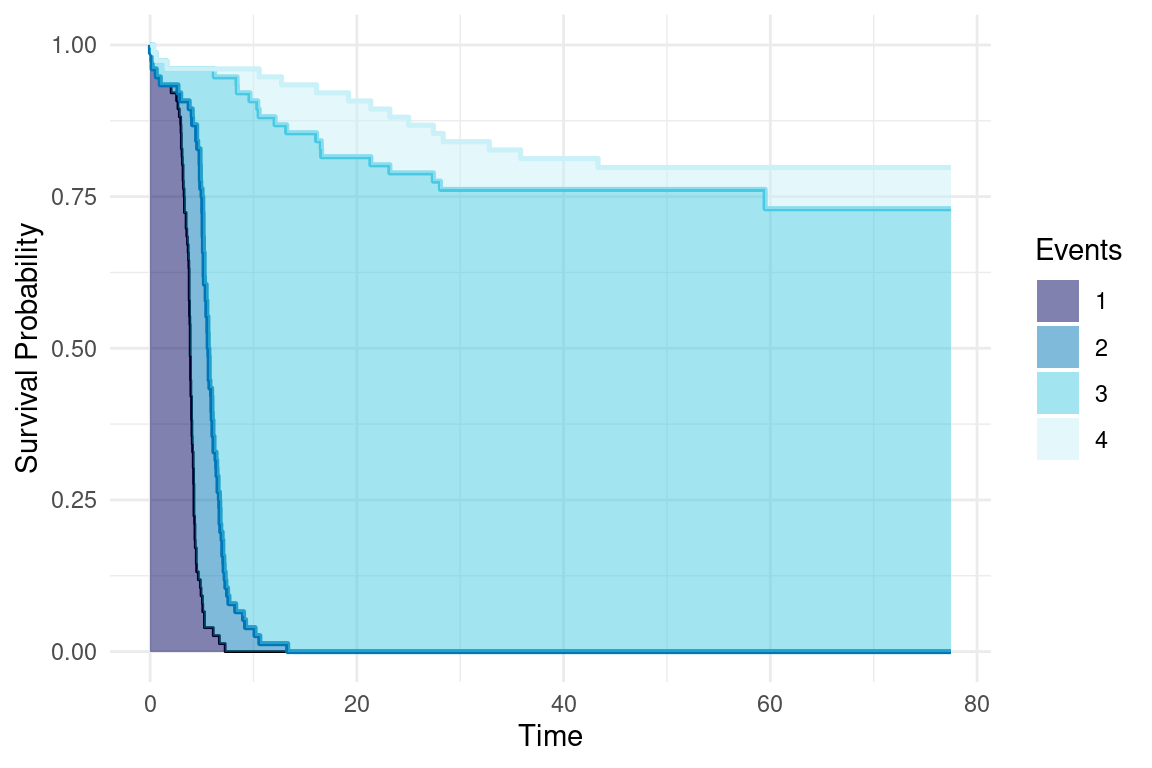
\includegraphics{partition_files/figure-latex/unnamed-chunk-11-1.pdf}

\begin{Shaded}
\begin{Highlighting}[]
\CommentTok{\# library(ggplot2)}
\CommentTok{\# \# Créer le graphique}
\CommentTok{\# ggplot(diff\_null, aes(x = uTOX, y = uREL)) +}
\CommentTok{\#   geom\_point() + }
\CommentTok{\#   scale\_x\_continuous(name = "Utility coefficient after relapse (μ\_REL)", limits = c(0, 1)) +}
\CommentTok{\#   scale\_y\_continuous(name = "Utility coefficient for toxicity (μ\_TOX)", limits = c(0, 1)) +}
\CommentTok{\#   geom\_abline(diffQTWiST1\_Diff, linetype = "dashed")}
\end{Highlighting}
\end{Shaded}

\hypertarget{threshold-analysis-for-q-twist-diff-with-bootstrapp-var-cov}{%
\subsubsection{Threshold analysis for Q-TWIST diff with bootstrapp
var-cov}\label{threshold-analysis-for-q-twist-diff-with-bootstrapp-var-cov}}

\begin{Shaded}
\begin{Highlighting}[]
\NormalTok{delta\_qtwist }\OtherTok{\textless{}{-}} \ControlFlowTok{function}\NormalTok{(data, indices, uTWiST, uTOX, uREL, t\_censure) \{}
\NormalTok{  sampled\_data }\OtherTok{\textless{}{-}}\NormalTok{ data[indices, ]}
  
  \CommentTok{\# Calculer les RMST pour chaque bras et chaque étape}
\NormalTok{  ct\_rmst }\OtherTok{\textless{}{-}} \FunctionTok{rmst2}\NormalTok{(sampled\_data}\SpecialCharTok{$}\NormalTok{delfinct, sampled\_data}\SpecialCharTok{$}\NormalTok{finct, }\FunctionTok{as.factor}\NormalTok{(}\FunctionTok{as.numeric}\NormalTok{(sampled\_data}\SpecialCharTok{$}\NormalTok{R1)}\SpecialCharTok{{-}}\DecValTok{1}\NormalTok{), }\AttributeTok{covariates =} \ConstantTok{NULL}\NormalTok{, }\AttributeTok{alpha =} \FloatTok{0.05}\NormalTok{)}
\NormalTok{  ct\_rmstB }\OtherTok{\textless{}{-}}\NormalTok{ ct\_rmst}\SpecialCharTok{$}\NormalTok{RMST.arm1}\SpecialCharTok{$}\NormalTok{rmst[}\DecValTok{1}\NormalTok{]}
\NormalTok{  ct\_rmstA }\OtherTok{\textless{}{-}}\NormalTok{ ct\_rmst}\SpecialCharTok{$}\NormalTok{RMST.arm0}\SpecialCharTok{$}\NormalTok{rmst[}\DecValTok{1}\NormalTok{]}
  
  \CommentTok{\# ct2\_rmst \textless{}{-} rmst2(sampled\_data$delfinct2, sampled\_data$finct2, as.factor(as.numeric(sampled\_data$R1){-}1), covariates = NULL, alpha = 0.05)}
  \CommentTok{\# ct2\_rmstB \textless{}{-} ct2\_rmst$RMST.arm1$rmst[1]}
  \CommentTok{\# ct2\_rmstA \textless{}{-} ct2\_rmst$RMST.arm0$rmst[1]}
  
\NormalTok{  sv\_rmst }\OtherTok{\textless{}{-}} \FunctionTok{rmst2}\NormalTok{(sampled\_data}\SpecialCharTok{$}\NormalTok{suivi, }\FunctionTok{as.numeric}\NormalTok{(}\FunctionTok{as.character}\NormalTok{(sampled\_data}\SpecialCharTok{$}\NormalTok{dc)), }\FunctionTok{as.factor}\NormalTok{(}\FunctionTok{as.numeric}\NormalTok{(sampled\_data}\SpecialCharTok{$}\NormalTok{R1)}\SpecialCharTok{{-}}\DecValTok{1}\NormalTok{), }\AttributeTok{tau =}\NormalTok{ t\_censure, }\AttributeTok{covariates =} \ConstantTok{NULL}\NormalTok{, }\AttributeTok{alpha =} \FloatTok{0.05}\NormalTok{)}
\NormalTok{  sv\_rmstB }\OtherTok{\textless{}{-}}\NormalTok{ sv\_rmst}\SpecialCharTok{$}\NormalTok{RMST.arm1}\SpecialCharTok{$}\NormalTok{rmst[}\DecValTok{1}\NormalTok{]}
\NormalTok{  sv\_rmstA }\OtherTok{\textless{}{-}}\NormalTok{ sv\_rmst}\SpecialCharTok{$}\NormalTok{RMST.arm0}\SpecialCharTok{$}\NormalTok{rmst[}\DecValTok{1}\NormalTok{]}
  
\NormalTok{  efs\_rmst }\OtherTok{\textless{}{-}} \FunctionTok{rmst2}\NormalTok{(sampled\_data}\SpecialCharTok{$}\NormalTok{delpfs, }\FunctionTok{as.numeric}\NormalTok{(}\FunctionTok{as.character}\NormalTok{(sampled\_data}\SpecialCharTok{$}\NormalTok{pfs)), }\FunctionTok{as.factor}\NormalTok{(}\FunctionTok{as.numeric}\NormalTok{(sampled\_data}\SpecialCharTok{$}\NormalTok{R1)}\SpecialCharTok{{-}}\DecValTok{1}\NormalTok{), }\AttributeTok{tau =}\NormalTok{ t\_censure, }\AttributeTok{covariates =} \ConstantTok{NULL}\NormalTok{, }\AttributeTok{alpha =} \FloatTok{0.05}\NormalTok{)}
\NormalTok{  efs\_rmstB }\OtherTok{\textless{}{-}}\NormalTok{ efs\_rmst}\SpecialCharTok{$}\NormalTok{RMST.arm1}\SpecialCharTok{$}\NormalTok{rmst[}\DecValTok{1}\NormalTok{]}
\NormalTok{  efs\_rmstA }\OtherTok{\textless{}{-}}\NormalTok{ efs\_rmst}\SpecialCharTok{$}\NormalTok{RMST.arm0}\SpecialCharTok{$}\NormalTok{rmst[}\DecValTok{1}\NormalTok{]}
  
  \CommentTok{\# Calculer les tox, twists et rels pour chaque bras et chaque étape}
\NormalTok{  tox1\_A }\OtherTok{\textless{}{-}}\NormalTok{ ct\_rmstA}
\NormalTok{  twist1\_A }\OtherTok{\textless{}{-}}\NormalTok{ efs\_rmstA }\SpecialCharTok{{-}}\NormalTok{ ct\_rmstA}
\NormalTok{  rel\_A }\OtherTok{\textless{}{-}}\NormalTok{ sv\_rmstA }\SpecialCharTok{{-}}\NormalTok{ efs\_rmstA}
  
\NormalTok{  tox1\_B }\OtherTok{\textless{}{-}}\NormalTok{ ct\_rmstB}
\NormalTok{  twist1\_B }\OtherTok{\textless{}{-}}\NormalTok{ efs\_rmstB }\SpecialCharTok{{-}}\NormalTok{ ct\_rmstB}
\NormalTok{  rel\_B }\OtherTok{\textless{}{-}}\NormalTok{ sv\_rmstB }\SpecialCharTok{{-}}\NormalTok{ efs\_rmstB}
  
  \CommentTok{\# Calculer les différences entre les bras}
\NormalTok{  tox1\_diff }\OtherTok{\textless{}{-}}\NormalTok{ tox1\_A }\SpecialCharTok{{-}}\NormalTok{ tox1\_B}
\NormalTok{  twist1\_diff }\OtherTok{\textless{}{-}}\NormalTok{ twist1\_A }\SpecialCharTok{{-}}\NormalTok{ twist1\_B}
\NormalTok{  rel\_diff }\OtherTok{\textless{}{-}}\NormalTok{ rel\_A }\SpecialCharTok{{-}}\NormalTok{ rel\_B}
  
  \CommentTok{\# Calculer QTWiST pour chaque partition}
\NormalTok{  q\_twist1\_A }\OtherTok{\textless{}{-}}\NormalTok{ (uTOX }\SpecialCharTok{*}\NormalTok{ tox1\_A) }\SpecialCharTok{+}\NormalTok{ (uTWiST }\SpecialCharTok{*}\NormalTok{ twist1\_A) }\SpecialCharTok{+}\NormalTok{ (uREL }\SpecialCharTok{*}\NormalTok{ rel\_A)}
\NormalTok{  q\_twist1\_B }\OtherTok{\textless{}{-}}\NormalTok{ (uTOX }\SpecialCharTok{*}\NormalTok{ tox1\_B) }\SpecialCharTok{+}\NormalTok{ (uTWiST }\SpecialCharTok{*}\NormalTok{ twist1\_B) }\SpecialCharTok{+}\NormalTok{ (uREL }\SpecialCharTok{*}\NormalTok{ rel\_B)}
\NormalTok{  q\_twist1\_diff }\OtherTok{\textless{}{-}}\NormalTok{ q\_twist1\_A }\SpecialCharTok{{-}}\NormalTok{ q\_twist1\_B}
  
  
  \CommentTok{\# Retourner les résultats}
  \FunctionTok{return}\NormalTok{(}\StringTok{"q\_TWiST1 diff"} \OtherTok{=}\NormalTok{ q\_twist1\_diff)\}}


\CommentTok{\# delta\_qtwist\_boot \textless{}{-} censboot(qaly\_cens, delta\_qtwist, R = 1000, uTWiST = 1, uTOX = 0.5, uREL = 0.5, t\_censure = t\_censure)}
\CommentTok{\# boot.ci(delta\_qtwist\_boot,type="norm")$normal}
\FunctionTok{library}\NormalTok{(boot)}
\CommentTok{\# QTWiST}
\NormalTok{results1 }\OtherTok{\textless{}{-}} \FunctionTok{data.frame}\NormalTok{(}\AttributeTok{uTOX=}\FunctionTok{numeric}\NormalTok{(), }\AttributeTok{uREL=}\FunctionTok{numeric}\NormalTok{(), }\AttributeTok{QTWiST1\_Diff=}\FunctionTok{numeric}\NormalTok{(), }\AttributeTok{Lower=}\FunctionTok{numeric}\NormalTok{(), }\AttributeTok{Upper=}\FunctionTok{numeric}\NormalTok{())}

\ControlFlowTok{for}\NormalTok{ (uTOX }\ControlFlowTok{in} \FunctionTok{seq}\NormalTok{(}\DecValTok{0}\NormalTok{, }\DecValTok{1}\NormalTok{, }\AttributeTok{by=}\FloatTok{0.25}\NormalTok{)) \{}
  \ControlFlowTok{for}\NormalTok{ (uREL }\ControlFlowTok{in} \FunctionTok{seq}\NormalTok{(}\DecValTok{0}\NormalTok{, }\DecValTok{1}\NormalTok{, }\AttributeTok{by=}\FloatTok{0.25}\NormalTok{)) \{}
    \CommentTok{\# Bootstrap analysis}
\NormalTok{    delta\_qtwist\_boot }\OtherTok{\textless{}{-}} \FunctionTok{censboot}\NormalTok{(qaly\_cens, delta\_qtwist, }\AttributeTok{R =} \DecValTok{1000}\NormalTok{, }\AttributeTok{uTWiST =}\NormalTok{ uTWiST, }\AttributeTok{uTOX =}\NormalTok{ uTOX, }\AttributeTok{uREL =}\NormalTok{ uREL, }\AttributeTok{t\_censure =}\NormalTok{ t\_censure)}
\NormalTok{    boot\_results }\OtherTok{\textless{}{-}} \FunctionTok{boot.ci}\NormalTok{(delta\_qtwist\_boot, }\AttributeTok{type=}\StringTok{"norm"}\NormalTok{)}
\NormalTok{    boot\_results}\SpecialCharTok{$}\NormalTok{normal[}\DecValTok{2}\NormalTok{]}
    \CommentTok{\# Ajouter les résultats dans le dataframe}
\NormalTok{results1 }\OtherTok{\textless{}{-}} \FunctionTok{rbind}\NormalTok{(results1, }\FunctionTok{data.frame}\NormalTok{(}
      \AttributeTok{uTOX=}\NormalTok{uTOX, }
      \AttributeTok{uREL=}\NormalTok{uREL, }
      \AttributeTok{QTWiST1\_Diff=}\NormalTok{q\_twist1\_diff, }
      \AttributeTok{Lower=}\NormalTok{boot\_results}\SpecialCharTok{$}\NormalTok{normal[}\DecValTok{2}\NormalTok{], }\CommentTok{\# Lower CI}
      \AttributeTok{Upper=}\NormalTok{boot\_results}\SpecialCharTok{$}\NormalTok{normal[}\DecValTok{3}\NormalTok{]  }\CommentTok{\# Upper CI}
\NormalTok{))}
\NormalTok{    \}}
\NormalTok{\}}
\end{Highlighting}
\end{Shaded}

\hypertarget{export-results-in-latex}{%
\subsection{Export results in latex}\label{export-results-in-latex}}

\begin{Shaded}
\begin{Highlighting}[]
\ControlFlowTok{if}\NormalTok{ (}\SpecialCharTok{!}\FunctionTok{require}\NormalTok{(}\StringTok{"xtable"}\NormalTok{)) }\FunctionTok{install.packages}\NormalTok{(}\StringTok{"xtable"}\NormalTok{)}
\end{Highlighting}
\end{Shaded}

\begin{verbatim}
## Le chargement a nécessité le package : xtable
\end{verbatim}

\begin{Shaded}
\begin{Highlighting}[]
\FunctionTok{library}\NormalTok{(xtable)}

\FunctionTok{rownames}\NormalTok{(results)}
\end{Highlighting}
\end{Shaded}

\begin{verbatim}
##  [1] "Est."   "Est.1"  "Est.2"  "Est.3"  "Est.4"  "Est.5"  "Est.6"  "Est.7" 
##  [9] "Est.8"  "Est.9"  "Est.10" "Est.11" "Est.12" "Est.13" "Est.14" "Est.15"
## [17] "Est.16" "Est.17" "Est.18" "Est.19" "Est.20" "Est.21" "Est.22" "Est.23"
## [25] "Est.24"
\end{verbatim}

\begin{Shaded}
\begin{Highlighting}[]
\FunctionTok{print}\NormalTok{(}\FunctionTok{xtable}\NormalTok{(results), }\AttributeTok{type =} \StringTok{"latex"}\NormalTok{, }\AttributeTok{include.rownames =} \ConstantTok{FALSE}\NormalTok{)}
\end{Highlighting}
\end{Shaded}

\begin{verbatim}
## % latex table generated in R 4.3.3 by xtable 1.8-4 package
## % Tue Apr  2 18:14:11 2024
## \begin{table}[ht]
## \centering
## \begin{tabular}{rrrrr}
##   \hline
## uTOX & uREL & QTWiST1\_Diff & Lower & Upper \\ 
##   \hline
## 0.00 & 0.00 & 7.73 & 0.42 & 15.04 \\ 
##   0.00 & 0.25 & 6.67 & -0.68 & 14.02 \\ 
##   0.00 & 0.50 & 5.61 & -1.91 & 13.14 \\ 
##   0.00 & 0.75 & 4.55 & -3.27 & 12.38 \\ 
##   0.00 & 1.00 & 3.50 & -4.74 & 11.74 \\ 
##   0.25 & 0.00 & 7.77 & 0.46 & 15.08 \\ 
##   0.25 & 0.25 & 6.71 & -0.64 & 14.06 \\ 
##   0.25 & 0.50 & 5.66 & -1.87 & 13.18 \\ 
##   0.25 & 0.75 & 4.60 & -3.23 & 12.42 \\ 
##   0.25 & 1.00 & 3.54 & -4.70 & 11.78 \\ 
##   0.50 & 0.00 & 7.82 & 0.50 & 15.13 \\ 
##   0.50 & 0.25 & 6.76 & -0.59 & 14.11 \\ 
##   0.50 & 0.50 & 5.70 & -1.83 & 13.23 \\ 
##   0.50 & 0.75 & 4.64 & -3.19 & 12.47 \\ 
##   0.50 & 1.00 & 3.58 & -4.66 & 11.83 \\ 
##   0.75 & 0.00 & 7.86 & 0.54 & 15.18 \\ 
##   0.75 & 0.25 & 6.80 & -0.55 & 14.16 \\ 
##   0.75 & 0.50 & 5.74 & -1.78 & 13.27 \\ 
##   0.75 & 0.75 & 4.69 & -3.14 & 12.52 \\ 
##   0.75 & 1.00 & 3.63 & -4.62 & 11.87 \\ 
##   1.00 & 0.00 & 7.90 & 0.58 & 15.22 \\ 
##   1.00 & 0.25 & 6.85 & -0.51 & 14.20 \\ 
##   1.00 & 0.50 & 5.79 & -1.74 & 13.32 \\ 
##   1.00 & 0.75 & 4.73 & -3.10 & 12.56 \\ 
##   1.00 & 1.00 & 3.67 & -4.58 & 11.92 \\ 
##    \hline
## \end{tabular}
## \end{table}
\end{verbatim}

\begin{Shaded}
\begin{Highlighting}[]
\CommentTok{\# \%\textgreater{}\% }
\CommentTok{\#   as\_gt()\%\textgreater{}\% }
\CommentTok{\#   gtsave("name.text")}
\end{Highlighting}
\end{Shaded}


\end{document}
